\documentclass[manuscript, review, screen]{acmart}


%\setcitestyle{super,sort&compress}
\usepackage{booktabs} % For formal tables

\usepackage[ruled]{algorithm2e} % For algorithms
\usepackage{array} 
\usepackage{wrapfig}
\usepackage{graphicx}
\usepackage{longtable}
\usepackage{lineno}
\usepackage{framed}
\usepackage{float}
\restylefloat{table}
\usepackage{rotating}
\usepackage{subfigure}
\usepackage{enumitem}
\usepackage{color}
%\usepackage[dvips]{color}

\usepackage{wrapfig}
\usepackage{longtable}
\usepackage{lineno}
\usepackage{framed}
\usepackage{float}
\restylefloat{table}
\usepackage{rotating}
%\usepackage{subfigure}
\usepackage{enumitem}
\usepackage{color}
\usepackage{framed}
\usepackage{colortbl}
\usepackage{amsmath}

% \usepackage[disable]{todonotes} % notes not showed
\usepackage[draft]{todonotes}   % notes showed


%\usepackage{subfigure}
\usepackage{tabularx}

\usepackage{url}
%\usepackage{xcolor}
%\usepackage[dvips]{color}
\usepackage{bbding}
\usepackage{url}
\usepackage{balance}
\usepackage{multirow}
\usepackage{booktabs}
\usepackage{graphicx}
\usepackage[framemethod=tikz]{mdframed}

\usepackage{amsmath}
\usepackage{amssymb}
\usepackage{graphicx}
\usepackage{rotating}
%\usepackage[table,xcdraw]{xcolor}
% *** GRAPHICS RELATED PACKAGES ***
%

\usepackage{amsmath}

% *** SPECIALIZED LIST PACKAGES ***
%
\usepackage{algorithmic}

\newmdenv[innerlinewidth=0.5pt, roundcorner=4pt,innerleftmargin=6pt,
innerrightmargin=6pt,innertopmargin=6pt,innerbottommargin=6pt]{mybox}

%\usepackage{subcaption}

\usepackage[ruled]{algorithm2e} % For algorithms
\renewcommand{\algorithmcfname}{ALGORITHM}
\SetAlFnt{\small}
\SetAlCapFnt{\small}
\SetAlCapNameFnt{\small}
\SetAlCapHSkip{0pt}
\IncMargin{-\parindent}

% Metadata Information
\acmJournal{CSUR}
\acmVolume{9}
\acmNumber{4}
\acmArticle{39}
\acmYear{2019}
\acmMonth{3}
\acmArticleSeq{11}

%\acmBadgeR[http://ctuning.org/ae/ppopp2016.html]{ae-logo}
%\acmBadgeL[http://ctuning.org/ae/ppopp2016.html]{ae-logo}


% Copyright
%\setcopyright{acmcopyright}
%\setcopyright{acmlicensed}
%\setcopyright{rightsretained}
%\setcopyright{usgov}
\setcopyright{usgovmixed}
%\setcopyright{cagov}
%\setcopyright{cagovmixed}

% DOI
\acmDOI{0000001.0000001}

% Paper history
\received{February 2019}
\received{March 2019}
\received[accepted]{June 2019}


% Document starts
\begin{document}
% Title portion
\title{Computing For Cybercrime Threat Intelligence:\\ a Systematic Multi-Vocal Literature Review}
%\titlenote{We can add a note to the title}

\author{Giuseppe Cascavilla}
\authornote{This is the corresponding author}
\affiliation{%
  \institution{Jheronimus Academy of Data Science}
  \city{'s-Hertogenbosch}
  \country{Netherlands}
}
\email{ g.cascavilla@tue.nl}

\author{Damian A. Tamburri}
\orcid{orcid number}
\affiliation{%
  \institution{Jheronimus Academy of Data Science} 
  \streetaddress{Sint Janssingel 92}
  \city{'s-Hertogenbosch}
  %\state{NL}
  \postcode{5211 DA}
  \country{Netherlands}}
\email{d.a.tamburri@tue.nl}

\author{Willem-Jan Van Den Heuvel}
\orcid{orcid number}
\affiliation{%
  \institution{Jheronimus Academy of Data Science}
  \streetaddress{Sint Janssingel 92}
  \city{'s-Hertogenbosch}
  %\state{NL}
  \postcode{5211 DA}
  \country{Netherlands}}
\email{w.j.a.m.v.d.heuvel@jads.nl}
% \author{Aparna Patel}
% \affiliation{%
%  \institution{Rajiv Gandhi University}
%  \streetaddress{Rono-Hills}
%  \city{Doimukh}
%  \state{Arunachal Pradesh}
%  \country{India}}
% \email{aprna_patel@rguhs.ac.in}
% \author{Huifen Chan}
% \affiliation{%
%   \institution{Tsinghua University}
%   \streetaddress{30 Shuangqing Rd}
%   \city{Haidian Qu}
%   \state{Beijing Shi}
%   \country{China}
% }
% \email{chan0345@tsinghua.edu.cn}
% \author{Ting Yan}
% \affiliation{%
%   \institution{Eaton Innovation Center}
%   \city{Prague}
%   \country{Czech Republic}}
% \email{yanting02@gmail.com}
% \author{Tian He}
% \affiliation{%
%   \institution{University of Virginia}
%   \department{School of Engineering}
%   \city{Charlottesville}
%   \state{VA}
%   \postcode{22903}
%   \country{USA}
% }
% \affiliation{%
%   \institution{University of Minnesota}
%   \country{USA}}
% \email{tinghe@uva.edu}
% \author{Chengdu Huang}
% \author{John A. Stankovic}
% \author{Tarek F. Abdelzaher}
% \affiliation{%
%   \institution{University of Virginia}
%   \department{School of Engineering}
%   \city{Charlottesville}
%   \state{VA}
%   \postcode{22903}
%   \country{USA}
% }



\begin{abstract}
Major cybersecurity and threat intelligence analysts agree that Online criminal activity is increasing exponentially. To offer an overview of the techniques and indicators to perform cybercrime detection and threat intelligence over multiple analysis levels (i.e., surface, deep, and darkwebs) we systematically analyse the state of the art in such techniques. We provide (1) a taxonomy of existing methods mapped to (2) an overview of detectable criminal activities as well as (3) an overview of the indicators and risk parameters that can be used for such detection. We conclude that both practitioners and academicians should effectively cooperate to address the emerging field, potentially harnessing a combination of the surveyed techniques.
\end{abstract}


%
% The code below should be generated by the tool at
% http://dl.acm.org/ccs.cfm
% Please copy and paste the code instead of the example below.
%
% \begin{CCSXML}
% <ccs2012>
%  <concept>
%   <concept_id>10010520.10010553.10010562</concept_id>
%   <concept_desc>Computer systems organization~Embedded systems</concept_desc>
%   <concept_significance>500</concept_significance>
%  </concept>
%  <concept>
%   <concept_id>10010520.10010575.10010755</concept_id>
%   <concept_desc>Computer systems organization~Redundancy</concept_desc>
%   <concept_significance>300</concept_significance>
%  </concept>
%  <concept>
%   <concept_id>10010520.10010553.10010554</concept_id>
%   <concept_desc>Computer systems organization~Robotics</concept_desc>
%   <concept_significance>100</concept_significance>
%  </concept>
%  <concept>
%   <concept_id>10003033.10003083.10003095</concept_id>
%   <concept_desc>Networks~Network reliability</concept_desc>
%   <concept_significance>100</concept_significance>
%  </concept>
% </ccs2012>
% \end{CCSXML}

% \ccsdesc[500]{Computer systems organization~Embedded systems}
% \ccsdesc[300]{Computer systems organization~Redundancy}
% \ccsdesc{Computer systems organization~Robotics}
% \ccsdesc[100]{Networks~Network reliability}

%
% End generated code
%


%\keywords{Add keywords here}

% DO NOT use this command unless you want to change
% the default behavior
% \authorsaddresses{Authors' addresses: G.~Zhou, Computer Science
%   Department, College of William and Mary, 104 Jameson Rd,
%   Williamsburg, PA 23185, US, \path{gzhou@wm.edu}; V.~B\'eranger,
%   Inria Paris-Rocquencourt, Rocquencourt, France; A.~Patel, Rajiv
%   Gandhi University, Rono-Hills, Doimukh, Arunachal Pradesh, India;
%   H.~Chan, Tsinghua University, 30 Shuangqing Rd, Haidian Qu, Beijing
%   Shi, China; T.~Yan, Eaton Innovation Center, Prague, Czech Republic;
%   T.~He, C.~Huang, J.~A.~Stankovic University of Virginia, School of
%   Engineering Charlottesville, VA 22903, USA; T. F. Abdelzaher,
%   (Current address) NASA Ames Research Center, Moffett Field,
%   California 94035.}

\maketitle

% The default list of authors is too long for headers.
%\renewcommand{\shortauthors}{Cascavilla et al.}
\section{Introduction}
\subsection{Vision and Scope}

Techopedia\footnote{\url{https://www.techopedia.com/definition/2387/cybercrime}} defines Cybercrime as ``[...] a crime in which a computer is the object of the crime (hacking, phishing, spamming) or is used as a tool to commit an offense (child pornography, hate crimes). Cybercriminals may use computer technology to access personal information, business trade secrets or use the internet for exploitative or malicious purposes. Criminals can also use computers for communication and document or data storage. Criminals who perform these illegal activities are often referred to as hackers". As a large-scale phenomenon, Cybercrime hit the headlines in 2017, with the likes of \emph{WannaCry} crippling the National Health Service in May that year, or the Petya/NotPetya ransomware attack infecting global companies shortly thereafter, with a whole host of data breaches from big companies like Equifax. The year 2018 suffered no better fate, indeed \cite{SolanoP17}. In total, the figures around the phenomenon~\footnote{as reported by the InformationAge online media conglomerate.} are staggering: (a) The global cost of Cyber Crime is estimated to reach \$2 trillion by 2019, a threefold increase from the 2015 estimate of \$500 billion; (2) The cost per record stolen averages \$158; (3) in 2018 there were 38\% more cyber-incidents than the previous year; (4) 48\% of crimes are caused with malicious intent --- human error or system failure account for the rest.
%https://www.zdnet.com/article/why-microsoft-is-fighting-to-stop-a-cyber-world-war/?ftag=TRE7ce1dc9&bhid=21378160878801111613213596198479

At the same time, \emph{threat intelligence} is the discipline whose intent is that of providing organized, analyzed, and refined information about potential or current attacks that threaten an organization, including governments, non-governmental organizations, and more \cite{TounsiR18}.

In this paper we aim at providing a synthesis of the state of the art in \emph{cybercrime} threat intelligence, accounting for both grey and white literature on the matter with a systematic \emph{multi-vocal} literature review \cite{slr,garousi2013evaluating}. 

Our results provide a clear overview of most if not all the topics, approaches, indicators, risks, fallacies, and pitfalls around the phenomenon. Our end goal is offering such an overview to encourage analysis, synthesis, and avoidance of the risks connected to cybercrime, starting from techniques existing in the state of the art. The impact of these results is considerable for both practitioners and academicians. On one hand, practitioners may benefit from our results in that they offer indicators, techniques, and tools that help avoiding the damage connected to the phenomenon; on the other hand, the synthesis offered in the following pages offers a starting basis to study the cybercrime phenomenon in deeper detail.

\subsection{Approach and Major Contributions}
%\begin{itemize}
%    \item overview of research questions with one line of methods to address each one
%    \item major contributions outline, with one line to explain the contribution, the intended user and practical impact
%\end{itemize}
Overall, our work focuses on addressing five research questions: (1) What online depth levels are assessed and to what extent?; (2) what degrees of anonymity exist for web-crawling?; (3) what policies exist to vary the degrees of anonymity?; (4) what website features are most indicative of cyberthreats?; (5) what risk assessment techniques exist?  Altogether, the research questions are aimed at shedding light over the approaches and techniques that could be combined into a risk-assessment campaign enacted by law-enforcement agencies (LEAs) or policy-makers over cybercrime perpetrated in novel online sources. Our theoretical assumption is that offering this background is vital to enact an educated design of proper risk-assessment technology stemming from previous work in the field.

The major contributions of this work are threefold: (a) a twin taxonomy for risk assessment in the surface and deep/darkweb; (b) a rigorously mined set of topics which can be used as quantitative indicators for  further risk assessment and confirmation; (c) a systematic overlap between contributions (a) and (b) to elaborated gaps in the state of the art and opportunities for further research.

\subsection{Structure of The Paper}

The rest of this paper is organized as follows. First, Sec. \ref{rel} outlines the background terms and definitions as well as outlining related work. Further on, Sec. \ref{mm} elaborates on the research design behind this study. Subsequently, Sec. \ref{res} outlines the results while Sec. \ref{disc} discusses them in context. Finally, Sec. \ref{conc} concludes the paper.

%\todo{to finish with the paragraphs}

\section{Background and Related Work}\label{rel}
To the best of our knowledge, this is the first systematic literature review providing a taxonomy about the different type of cybercrime and threat intelligence solutions. However, in the following paragraph, we are discussing some papers that provide a partial overview of threat intelligence rather than cybercrime risks or guidance note in order to assist to address the problem posed by cybercrime. In the online literature there are no surveys trying to create a general overview of the cybersecurity risks and the proposed solutions in order to contain the risks. Our systematic literature review analyses the state of the art of the upcoming cybersecurity risks and the proposed countermeasures today available.
Due to the novelty of the cybersecurity threats and the lack of technologies available to fight the cyber attacks, we will examine also sources from the web like blogs and news, in order to have a broader point of view on the new cybercrime trends.


\subsection{Terms and Definitions}
%\todo[fancyline]{we need to add references to each of the elements in the table 1 and also link the table somewhere in the text... else it is dangling! Furthermore, why these terms? we should explain the selection} 


Table~\ref{tab:definitions} lists all the terms and the related definitions used in this study. The table provides on the first column \textit{Terms} the list of those terms considered more technical and more cybersecurity/cybercrime related. On the second column \textit{Definitions} we provide a short explanation of the terms related to the cybersecurity environment. We provide this table in order to help the reader to better understand the whole work, indeed, some of the listed technical words are used in our study, meanwhile other terms could be useful in order to have a better background of the cybersecurity problem we are discussing.


\begin{table}[h!]
\small
%\begin{tabular}{@{}ll@{}}
%\begin{tabular}{ll}
\begin{tabular}{p{0.22\textwidth}p{0.74\textwidth}}
\toprule
\textbf{Terms} & \textbf{Definition} \\ \midrule
\rowcolor[HTML]{EFEFEF} 
Cyber Crime & \begin{tabular}[c]{@{}l@{}} Cybercrime is defined as a crime in which a computer is the object of the crime (hacking, \\phishing, spamming) or is used as a tool to commit an offense (child pornography, hate crimes) \cite{techopedia}.\end{tabular} \\
Surface Web & \begin{tabular}[c]{@{}l@{}}Surface web is the normal web which is visible for all users using internet. The websites in the\\ surface web is indexed by search engines. Google is the great example of search engine \cite{surfacewebdef}.\end{tabular} \\
\rowcolor[HTML]{EFEFEF} 
Deep Web & \begin{tabular}[c]{@{}l@{}}Deep web is the private web which is not visible for normal user. The deep web consist of\\ a website or any page on the website which are not indexed by search engines \cite{surfacewebdef}.\end{tabular} \\
Dark Web & \begin{tabular}[c]{@{}l@{}}The all criminal activities are act upon on dark web. The criminal activities like drugs dealing,\\ killing humans etc. The user can only access it if the user has Tor Browser \cite{surfacewebdef}.\end{tabular} \\
\rowcolor[HTML]{EFEFEF} 
Threat Intelligence & \begin{tabular}[c]{@{}l@{}}Is an organized, analyzed and refined information about potential or current attacks that threaten\\ an organization. The primary purpose of threat intelligence is helping organizations understand\\ the risks of the most common and severe external threats \cite{tintelligence}.\end{tabular} \\
\begin{tabular}[c]{@{}l@{}}Open Source Intelligence\\ (OSINT)\end{tabular} & \begin{tabular}[c]{@{}l@{}}Is the insight gained from processing and analyzing public data sources such as broadcast TV\\ and radio, social media, and websites. These sources provide data in text, video, image, and audio\\ formats \cite{OSINT}.\end{tabular} \\
\rowcolor[HTML]{EFEFEF} 
Crawler & \begin{tabular}[c]{@{}l@{}}A crawler is a program that visits Web sites and reads their pages and other information in order\\ to create entries or retrieve data \cite{crawler}.\end{tabular} \\
Malware & \begin{tabular}[c]{@{}l@{}}Or ``malicious software'', is an umbrella term that describes any malicious program or code that\\ is harmful to systems. Hostile, intrusive, and intentionally nasty, malware seeks to invade,\\ damage, or disable computers, computer systems, networks, tablets, and mobile devices, often\\ by taking partial control over a device's operations. Like the human flu, it interferes with normal \\functioning \cite{malware}.\end{tabular} \\
\rowcolor[HTML]{EFEFEF} 
\begin{tabular}[c]{@{}l@{}}Distributed Denial of Service \\ (DDoS)\end{tabular} & \begin{tabular}[c]{@{}l@{}}A distributed denial-of-service (DDoS) attack is an attack in which multiple compromised\\ computer systems attack a target, such as a server, website or other network resource, and cause\\ a denial of service for users of the targeted resource. The flood of incoming messages, connection\\ requests or malformed packets to the target system forces it to slow down or even crash and \\shut down, thereby denying service to legitimate users or systems \cite{ddosdef}.\end{tabular} \\
Watering Hole Attack & \begin{tabular}[c]{@{}l@{}}A watering hole attack is a security exploit in which the attacker seeks to compromise a specific \\group of end users by infecting websites that members of the group are known to visit. The goal\\ is to infect a targeted user's computer and gain access to the network at the target's place of\\ employment \cite{wholeatt}.\end{tabular} \\
\rowcolor[HTML]{EFEFEF} 
Spoofing & \begin{tabular}[c]{@{}l@{}}Is a fraudulent or malicious practice in which communication is sent from an unknown source \\disguised as a source known to the receiver. Spoofing is most prevalent in communication\\ mechanisms that lack a high level of security \cite{spoof}.\end{tabular} \\
Honeypot & \begin{tabular}[c]{@{}l@{}}A honeypot is a decoy computer system for trapping hackers or tracking unconventional or new\\ hacking methods. Honeypots are designed to purposely engage and deceive hackers and identify\\ malicious activities performed over the Internet \cite{hpot}.\end{tabular} \\
\rowcolor[HTML]{EFEFEF} 
Insider Threat & \begin{tabular}[c]{@{}l@{}}Insider threat is a generic term for a threat to an organization's security or data that comes \\from within. Such threats are usually attributed to employees or former employees, but may \\also arise from third parties, including contractors, temporary workers or customers \cite{insthreat}.\end{tabular} \\
\begin{tabular}[c]{@{}l@{}}Man-in-the-Middle Attack \\ (MITM)\end{tabular} & \begin{tabular}[c]{@{}l@{}}A man-in-the-middle (MITM) attack is a form of eavesdropping where  communication between\\ two users is monitored and modified by an unauthorized party \cite{mitm}.\end{tabular} \\
\rowcolor[HTML]{EFEFEF} 
Hacktivism & \begin{tabular}[c]{@{}l@{}}Hacktivism is the act of hacking a website or computer network in an effort to convey a social \\or political message. The person who carries out the act of hacktivism is known as a hacktivist \\\cite{Hacktivism}.\end{tabular} \\
\bottomrule
\end{tabular}
\caption{Definition of the terms from the survey paper.}
\label{tab:definitions}
\end{table}



\subsection{Related Surveys}

In a deeply connected world, like the one we are facing nowadays, hackers are constantly finding new targets and refining the tools they use to break through cyberdefenses. Moreover, the lack of privacy and security of the new upcoming technologies and the lack of awareness of the users poses a real threat to our personal life. In the following, we present some works that face the problem of cybersecurity and try to discuss the countermeasures today available. 

Tounsi et al. in \cite{TounsiR18} provide an overview of the open source/free threat intelligence tools and compare their features with those from AlliaCERT TI\footnote{Managed Security Services Division, AlliaCERT Team, Alliacom, France}. Through their analysis, they found that the fast sharing of threat intelligence, as encouraged by any organization in order to cooperate, is not enough to avoid targeted attacks. Moreover, trust is extremely important for companies that are sharing personal information. Another problem is how much data is important to share in order to prevent attacks and cooperate and in which format in order to avoid to lose information. In order to understand which standard is better Tounsi et al. propose their own analysis. Lastly, the work presents a comparison among the best threat intelligence tools dividing them in tools which privilege standardization and automatic analytics and others that focus on high speed requirements. 

Furthermore, If Tounsi et al. focus on what is the best way to keep the trust among organizations and at the same time share information about cyber threats, in Toch et al. \cite{Toch:2018:PIC:3186333.3172869} the authors pose the accent on the type of data required from those cybersecurity systems that are supposed to protect our privacy from prying eyes. The taxonomy suggested in the article shows that almost all cyber-security technological categories require some access to personal sensitive information. This result can offer guidance not only in choosing one technique over another but, more importantly, in designing more privacy-aware cyber-security technologies with little or no compromise with regard to their effectiveness in protecting from cyber attacks. 

The studies from above tried to analyze systems and good practices to mitigate the cyber threats, in Chang et al. \cite{ChangVWL13} we have a study regarding the state-of-the-art of web-based malware attacks and how to defense against. The paper starts with a study of the attack model and the vulnerabilities that enable these attacks, then analyzes the current state of the malware problem, lastly investigates the defense mechanisms. As result, the paper gives three categories of approaches in order to analyze, identify, and defend against the web-based malware problem. Each category with advantages and disadvantages and how these approaches complement each other and how they can work together. 

An altogether different approach from the previous ones is presented in Xu et al. \cite{Xu:2013:CDM:2435349.2435366} where the authors analyze network-layer traffic and application-layer websites contents simultaneously in order to detect the malicious web applications at run-time. The currently available approach to detect malicious websites can be classified into two categories: \textit{static approach} and \textit{dynamic approach}. The first approach analyzes URLs and contents the latter uses clients honeypots to analyze run-time behaviours. The results of this approach showed that cross-layer detection can achieve the same detection effectiveness of the dynamic approach, however it resulted to be much more faster than the dynamic one. 

In order to understand the rising concern around the cybersecurity problem another important reference is also the \emph{Guidance Note}\footnote{Link: \href{}{https://bit.ly/2BIy0tP}} of the United Nations Office on Drugs and Crime (UNODC) that is a global leader in the fight against illicit drugs and international crime. The guidance note aims at giving an overview about the most common cyber security threats today's available. Cybercrimes activities like the online radicalization, or the illicit sales of pharmaceutical solutions rather then frauds and identity theft are presented and explained in order to outline how UNODC can deliver technical assistance in order to address the problems posed by cybercrime at both regional and national levels.
If from scientific literature side we are seeing a huge growing of interest around cybersecurity threats, on the web side we have a lot of blogs and web-pages warning about the new upcoming cybersecurity threats. 

Furtheremore, we refer to reports of one of the major companies working in cybersecurity: Kaspersky\footnote{Link: \href{}{https://www.kaspersky.com}}. On the Kaspersky Threats blog page\footnote{Link: \href{}{https://bit.ly/2AijYiF}} where the company offers an updated list of the new upcoming cyber threats. More specifically, for example, on the top five worst cybersecurity attacks we have WannaCry and NotPetya/ExPetr two famous ransomware encryptor that use to encrypt the data of the victim user. Stuxnet a worm that targets the types of industrial control systems (ICS) that are commonly used in infrastructure supporting facilities (i.e. power plants, water treatment facilities, gas lines, etc). DarkHotel a spyware in order to conduct targeted phishing attacks using the hotel's Wi-Fi networks. In addition, Mirai is a botnet used to flood the DNS service provider Dyn with requests. The Kaspersky company gives guidelines \cite{kaspersky} on how address incident response in order to contain a cybersecurity attack. Kaspersky listed some key-points necessarily for a company to avoid and contain attacks: \emph{(i)} the speed a rapid remediation is key to limiting the costs, \emph{(ii)} proactive protection, \emph{(iii)} presence Of internal specialists. However, in order to have an world wide overview about real time cyber attacks, Kaspersky provided the Cyberthreat Real-Time Map available here \href{}{https://cybermap.kaspersky.com/} where is possible to see the current cyber attacks around the globe. 

Althogether, however, although plenty of white/grey literature exists on the topic, a holistic view over what software, indicators, methods, tools, and approaches to cyber-crime fighting that practitioners and law-enforces can use is still nowhere to be seen. We offer an initial attempt at such a review in the coming pages, for the benefit of practitioners and academicians alike.

%Anoter relevant related work in terms of cyber-threat intelligence is also the grey literature in the MIT series \cite{MIT} from M. Giles, a blog-site where the author lists and explains six major cybersecurity threats. \emph{Data breaches}, companies store a lot of personal and sensitive data, Marc Goodman, a security expert, thinks that people's personal web browsing habits will be the next popular targets. \emph{Ransomware in the cloud}, one big target in 2018 will be cloud computing businesses, which store a lot of data for companies. Subsequently, \emph{The weaponization of AI} entails AI driven arms to be supported by machine-learning models in order to better anticipate attacks. Hackers could take advantage of this to drive more phishing attacks. \emph{Cyber-physical attacks}, the new attacks could involve electrical grids, transportation systems, and other parts of countries' critical infrastructure. \emph{Mining cryptocurrencies} the act of mining needs a vast amounts of computing capacity to solve complex mathematical problems. This could encourage hackers to compromise computers in order to use them. \emph{Hacking election} fake news and cyberattacks on the voting process could be the next (?) threat we will face of. 
Another major company working in cybersecurity is Norton\footnote{Link: \href{}{https://us.norton.com/}}. In \cite{norton} a Symanthec employee gives a pictures of cybersecurity threats and the impact they have on the American population. Mobile malware and Third-party app stores seem to be the new concern. Spyware, ransomware, and viruses used to focus on laptop or desktop computer, however since 2017 the malware variants for mobile increased 54 percent. As well, Symantec, found third-party app stores hosted 99.9 percent of discovered mobile malware. From the Symantec report we can read that in 2023 cybercriminals will steal an estimated 33 billion records that might include your name, address, credit card information, or Social Security number. The impact of this identity theft will impact 60 million Americans and the average costs have been estimated in \$3.86 million (U.S. dollars) for the companies worldwide and \$7.91 million (U.S. dollars) for the U.S. company.
Our survey study try to create an overview among cyberthreats providing a taxonomy of the current criminal activities and complementary we provide on overview of indicators and risks parameters in order to detect cyber crime activities. To the best of our knowledge this is the first systematic literature review on cybersecurity and threat intelligence.



\section{Research Materials and Methods}\label{mm}
This systematic literature review seeks to address the research problem of providing a clear and detailed overview of the methods and indicators that can be used for cybercrime threat intelligence. Because much work has been conducted and disseminated in non-scientific venues and by non-governmental organisations, we opt for a systematic \emph{multivocal} literature review \cite{mv}, meaning that both grey and white literature are considered as equal sources of valuable data. In the rest of the section we flesh out the research questions and methods that we employed to attain our results.

\subsection{Research Questions and Approach}

To address the aforementioned topic we formulate the following master research question:
\begin{center}
    \textbf{MRQ.} \emph{what guidelines, methods, and principles exist to establish cyberthreat level of online sources?}
\end{center}

Furthermore, to make the MRQ manageable from a scientific and empirical inquiry perspective, we elaborate further on the master question using the following sub-research questions (SRQs), specifically:
\begin{enumerate}
\item [SRQ1.] what online depth levels are assessed and to what extent?
\item [SRQ2.] what degrees of anonymity exist for web-crawling?
\item [SRQ3.] what policies exist to vary the degrees of anonymity?
\item [SRQ4.] what website features are most indicative of cyberthreats?
\item [SRQ5.] what risk assessment techniques exist?
\item [SRQ6.] what data sources exist and how are they classified?
\end{enumerate}

The SRQs were designed to exhaustively cover the conceptual space reflected by our master research question. More specifically, in terms of SRQ1, we aim at figuring out which analysis techniques exist that cover which level of depth. Furthermore, in the scope of SRQ2 and SRQ3, we aim at understanding the techniques and approaches that would allow a law-enforcer to crawl online sources anonymously and to what extent this phenomenon is understood and addressed in the literature. Beyond that, with SRQ4 and SRQ5, we aim at figuring out which detection and analysis techniques exist and how they can be used, that is, upon which data features \cite{Zave03}. Finally, SRQ6 aims at cover the insights and intelligence available in the literature to describe and elaborate on the types and indicators around online sources of cybercrime (e.g., sites, blog-posts, APIs, etc.).

A major intrinsic difficulty of our study is our necessary reliance over what is called \emph{grey} literature~\cite{GarousiFM16}, intended as materials and research produced by organizations outside of the traditional commercial or academic publishing and distribution channels. Common grey literature publication types include reports (annual, research, technical, project, etc.), working papers, government documents, white papers and evaluations. On the one hand, the use of grey literature is risky since there is often little or no scientific factual representation of data or analyses presented in grey literature itself~\cite{schopfel2010literature}. 
On the other hand, a growing interest around using grey literature for computing practitioners' benefit as well as combining it to determine the state of the art and practice around a topic is gaining a considerable interest in many fields~\cite{schopfel2010literature,stempfhuber2008enhancing}, including software-related fields~\cite{GarousiFM16}.

For the scope of this study, and in an effort to maximize its validity, we followed a systematic approach based on the guidelines provided by Petersen et al.~\cite{sms-petersen} for conducting systematic literature reviews in software engineering. 
We hereby outline such a systematic approach,  starting from problem definition and describing the triangulation as well as other inter-rater reliability assessment trials we ran to enforce the validity of our findings.

Grey literature studies can typically be identified by exploiting search strings on search engines, with Google being the most prominent example.
Following the guidelines provided by Petersen et al.~\cite{sms-petersen}, we identified the search string by structuring them guided by our research questions.
More precisely, we defined the search strings based on the PICO terms of our question~\cite{kitchenham-charters}, by exploiting only the terms {\em Population} and {\em Intervention}.
The keywords %for our search 
were taken from each aspect of a research question. More specifically, the following search query was used:
%Differently from Petersen et al.~\cite{sms-petersen}
%, we did not restrict our focus to specific outcomes or experimental designs in our study, as we wished to have a broader overview of the industrial state-of-practice on microservices.
%By restricting ourselves to certain types of studies, we could have obtained a biased/incomplete analysis, as some sub-topics might have been over-/under-represented for certain types of study.
%The above explained difference is also reflected by the strings we employed for searching for the pains of microservices, viz.,
\\
\hspace*{\fill}
$
(\texttt{cyber*} \vee \texttt{online*}) \wedge (\texttt{threat*} \vee \texttt{attack*} \vee \texttt{activity*} \vee \texttt{crime*}) \wedge (\texttt{Surface*} \vee \texttt{D*})
$
\hspace*{\fill}
\\

In the above, the "$\texttt{*}$" symbol is the star wildcard which matches lexically-related terms (e.g.,~plurals, verb conjugations).

We exploited the above indicated search strings to look for industrial, government, and non-governmental studies (e.g.,~blog posts, whitepapers, industry-oriented magazines) that were published since the beginning of the internet until the mid of 2018. 
The search engines we employed are Google (primary), Bing, Duck Duck Go, Yahoo! and Webopedia.  Since engines look for the above indicated search strings over the whole pages they index, our search resulted in a high number of irrelevant studies, which were further refined with a secondary search and manual screening, based on the inclusion/exclusion criteria and control factors discussed in the following section. 

Similarly, to cover for white literature appropriately, we run the aforementioned query in typical and most common computing literature liberaries, namely: (1) ACM Digital Library; (2) IEEEXplore; (3) Wiley Interscience; (3) Elsevier Scopus; (4) Bibsonomy.

\subsection{Sample Selection \& Control Factors}
\label{sec:control-framework}
Table~\ref{tab:criteria} outlines the inclusion and exclusion criteria adopted in our sample selection.
%
% \begin{table}
% \caption{Inclusion/Exclusion criteria - an outline.}\label{criteria}
% \small
% \begin{tabular}{|>{\centering}p{2cm}|>{\centering}p{11,2cm}|}
% \hline 
%  & The study discusses the industrial application of microservices.\tabularnewline
% \cline{2-2} 
%  & The study discusses the benefits or shortcomings of microservice
% design and/or operation.\tabularnewline
% \cline{2-2} 
% Inclusion Criteria & The study reports on industrial direct experiences, educated practitioner
% opinions or otherwise practice around microservices.\tabularnewline
% \cline{2-2} 
%  & The study captures a practical case-study of microservices design
% and/or operation.\tabularnewline
% \cline{2-2} 
%  & The study describes business insights or losses connected to the
% use of microservices.\tabularnewline
% \hline 
%  & The study does not offer implementation details.\tabularnewline
% \cline{2-2} 
%  & The study does not offer design details.\tabularnewline
% \cline{2-2} 
% Exclusion Criteria & The study is not referred to industrial cases or other factual evidence.\tabularnewline
% \cline{2-2} 
%  & The study claimed benefits or pitfalls are not quantifiable.\tabularnewline
% \cline{2-2} 
%  & The study does not offer scope and limitations of proposed solutions,
% frameworks, patterns, tools.\tabularnewline
% \cline{2-2} 
%  & The study does not offer evidence of a practitioner perspective.\tabularnewline
% \hline 
% \end{tabular}
% \end{table}
%
\begin{table}[t]
\centering
\footnotesize
\begin{tabular}{p{0.1\textwidth}p{0.8\textwidth}}
\hline
	{\bf Case}
	&
    {\bf Criteria}
    \\
\hline
\rowcolor[HTML]{EFEFEF} 
	Inclusion 
    & 
	$\mathsf{i}_1$) The study discusses cybercrime or an application of analysis to the topic.\newline
	$\mathsf{i}_2$) The study discusses the ramifications and challenges around the topics close to our RQs.\newline
	$\mathsf{i}_3$) The study reports on direct experiences, opinions or practices on said topics by educated practitioners.\newline
	$\mathsf{i}_4$) The study refers to a practical case-study of design, development or operation of cybercrime threat intelligence approaches.
    \\
 	Exclusion 
    &
    $\mathsf{e}_1$) The study does not offer details on design or implementation of practices, methods, tools or indicators for cybercrime threat intelligence.\newline
	$\mathsf{e}_2$) The study is not referred to industrial cases or other factual evidence.\newline 
    $\mathsf{e}_3$) The benefits or pitfalls of discussed topics are not justified/quantified by the study.\newline
    $\mathsf{e}_4$) The study does not offer scope and limitations of proposed solutions, frameworks, patterns, tools.\newline 
    $\mathsf{e}_5$)The study does not offer evidence of a practitioner perspective.
 \\
\hline
\end{tabular}
\caption{Inclusion and exclusion criteria for sample selection.}
\label{tab:criteria}
\label{criteria}
\end{table}
%
The inclusion criteria ($\mathsf{i}_1 - \mathsf{i}_4$) were designed to focus explicitly on the kind of practical grey literature that identifies the targets of our study.
At the same time, the exclusion criteria permit disqualifying studies that do not offer the necessary design/implementation details ($\mathsf{e}_1$), that refer to nonfactual or unquantifiable evidence ($\mathsf{e}_2$ and $\mathsf{e}_3$), and that do not discuss the limitations and practical impact for the proposed solutions or outlined issues ($\mathsf{e}_4$ and $\mathsf{e}_5$). 
A study is to be selected if it satisfies {\em all} the inclusion criteria, while it is to be excluded if it satisfies at lease one of the exclusion criteria. % excluded articles It should be noted that articles in our sample reflect *all* the inclusion criteria, while excluded articles needed satisfy at least one of the exclusion criteria to warrant disqualification.

In addition to the inclusion/exclusion criteria in Table~\ref{criteria}, to ensure the quality of the selected grey literature, we selected only those industrial studies that were satisfying the following control factors:
\begin{enumerate}
\item \textbf{Practical Experience.} A study is to be selected only if it is written by practitioners with 5+ experience in the topic in object, or if it refers to established threat intelligence solutions with 2+ years of operation.
\item \textbf{Industrial Case-Study.} A study is to be selected only if it refers to at least 1 industrial case-study where a quantifiable number of threat intelligence tools are operated.
\item \textbf{Heterogeneity.} The selected studies reflect at least 5 top industrial domains and markets where threat intelligence tools were successfully applied.
\item \textbf{Implementation Quantity.} The selected studies refer to/show implementation details for the benefits and pitfall they discuss, so that other researchers and practitioners can use them in action.
\end{enumerate}

%\comment{JS}{We should mention (in this section?) which papers we identified (by pointing to the papers \s{1}-\s{37} listed in the Appendix \ref{sec:grey-literature})}

At the end of our screening, 374 studies were selected based on the inclusion/exclusion criteria and on the additional control factors. 
The complete list of selected studies is provided online~\footnote{\url{https://tinyurl.com/ANITAstudysourcesMSLR}}.

\subsection{Analysis Approach \& Inter-Rater Reliability Assessment}\label{sec:inter-rater-assessment}

To attain the findings we adopted a mixed-methods analysis approach \cite{JohOnw04}. 

\subsubsection{Thematic Coding}

To address SRQs 1-3 and 5-6, we adopted thematic coding~\cite{Bas03} to elicit a baseline understanding of the state of the art. More specifically, The selected sample of articles were subject to annotation and labeling with the goal of identifying themes emerging from the analyzed text. 
This process of analysis was executed in parallel over two 50\% splits of the entire dataset, to ensure avoidance of observer bias. 
The coders of the two splits (viz.,~the first two authors of this study) were then inverted and an inter-rater evaluation was enacted between the two emerging lists of themes. To evaluate inter-rater reliability, we adopted the widely known and adopted Krippendorff $\alpha$ coefficient (or K$\alpha$), which measures the agreement between two ordered lists of codes applied as part of content analysis \cite{content}. As part of our evaluation, K$\alpha$ was applied twice. 
\begin{itemize}
\item We applied the evaluation coefficient to measure the agreement between the two emerging lists of codes by the two independent observers who individually coded 100\% of the dataset in 2 rounds.
The result of applying K$\alpha$ to measure the agreement between these two lists amounted to 0.71, slightly lower than the typical reference score of 0.80 (i.e., 80\% agreement). A discussion and analysis of disagreement points revealed misalignment between the depth of the coding strategy, which was subsequently addressed; this modification brought the agreement between the emerging lists of codes to K$\alpha$ = 0.83.
\item K$\alpha$ was them applied again to triangulate the 0.83 score for the final list of themes with its identical counterpart, coded by the third author of this paper, who re-coded the entire dataset with the final coding strategy. The agreement between the final list A (obtained by the first 2 authors) and a final list B (obtained by the third author) was evaluated to K$\alpha$ = 0.93.
\end{itemize}

\subsubsection{Topic Modelling}

To address SRQ4, we operated a machine-assisted topic modelling and analysis exercise supported with a thematic coding. More specifically, we used Latent Dirichlet Allocation (LDA) to provide emerging themes in our textual data, subsequently labelling the emerging themes which are visible and observable characteristics of potential online sources for criminal activity (e.g., darknet websites). The application of LDA was carried out after standard text-mining pre-processing aimed at improving results by removing unnecessary information. Specifically: (1) all terms and definitions for the factors were standardised in terms of structure (i.e., definition + sample text extracted from reference papers); (2) punctuation marks and numbers were  removed; (3) all letters were converted to lower case; (4) all common stop words for English grammar and syntax were  removed.

For the afore-mentioned topic modelling exercise, we selected log-likelihood as our measure of clustering quality, following typical approaches from the state of the art \cite{AgrawalFM16}. In our case, however, the number of clusters started from typically used numbers adopted in the state of the art (k = 10 clusters) but the number was increased until at least one of the newly-emerging clusters contained less than half of the mean population of factors in the previous round. This approach was aimed at allowing the extraction of cybercrime activities and indicators that were meaningful, i.e., they reflected semantic commonalities among factors. In addition, We used the genetic algorithm Differential Evolution to tune LDA hyperparameters alpha and beta as suggested by Agrawal et al. \cite{AgrawalFM16}. To conduct all the above pre-processing and analyses we exploited the NetCulator bibliometric analytics tool\footnote{\url{https://www.netculator.com/}} which supports LDA and a number of similar natural-language analyses and clustering techniques and tools of our own design, featuring Python and the python LDA package.

%\subsection{Analysis Methods}


\section{Results}\label{res}
This section elaborates on our results starting from an overview of a randomly-selected, statistically-relevant subset (i.e., 20\% of the total of 374 papers) of the attained data-sources and their statistical distribution over a number of control factors. Subsequently, the section elaborates on findings from the study matching our sub-research questions from the Surface-, Deep- and dark-web perspectives, respectively.

\subsection{Dataset Descriptive Statistics}

\begin{figure}
\begin{center}
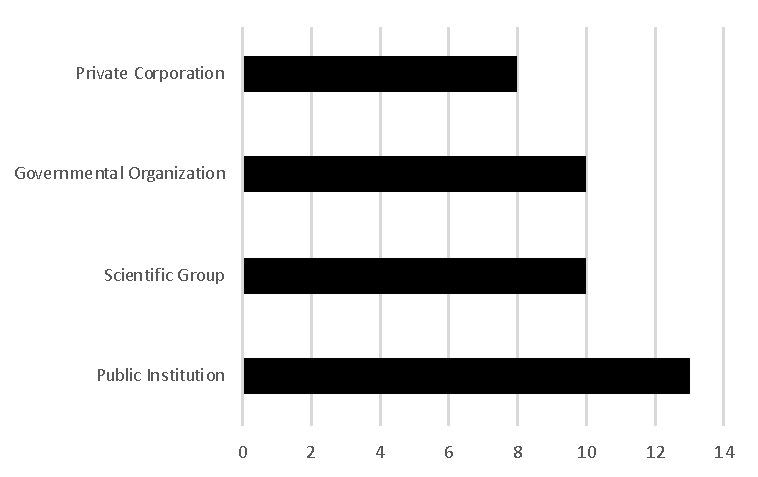
\includegraphics[scale=0.7]{./img/gcorptype}
\end{center}
\caption{types of organizations involved in the grey-literature, a majority of public organizations are involved.}\label{g1}
\end{figure}

The primary sources we reported offer a diverse statistical distribution over the last 20+ years. Figures from \ref{g1} to \ref{g3} outline statistical descriptors for the elicited grey literature while Figures \ref{w1} to \ref{w3} offer a similar insight into white literature. More specifically, Fig. \ref{g1} outlines the types of organisations who conducted the research reported in our primary studies, ranging from private corporations (e.g., Kaspersky labs) to public institutions (e.g., non-governmental organizations and boards), who cover for the majority of our sample. Further on, Fig. \ref{g2} provides a timeline reflecting a linear increase in interest over the phenomenon between the oldest (2006) and newest (2018) article we analysed while Fig. \ref{g3} provides a deeeper insight into the types of evaluations conducted in the grey-literature in question, with a striking majority of experience reports being used as basis for argument.

\begin{figure}
\begin{center}
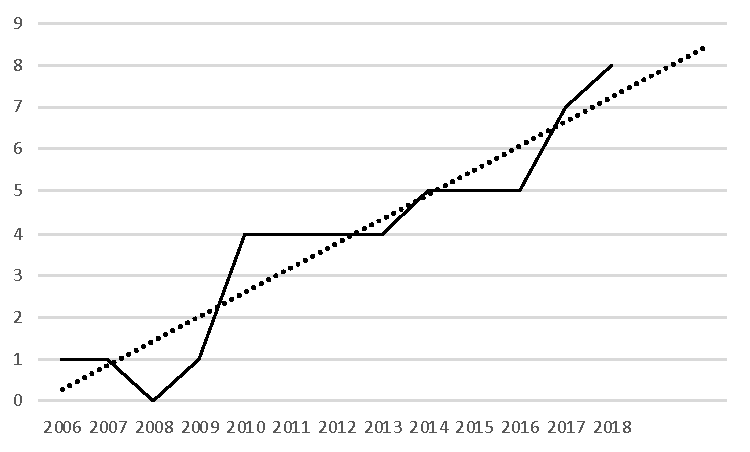
\includegraphics[scale=0.7]{./img/gtimeline.pdf}
\end{center}
\caption{increase of interest over the topic; a linear increase is reported.}\label{g2}
\end{figure}

\begin{figure}
\begin{center}
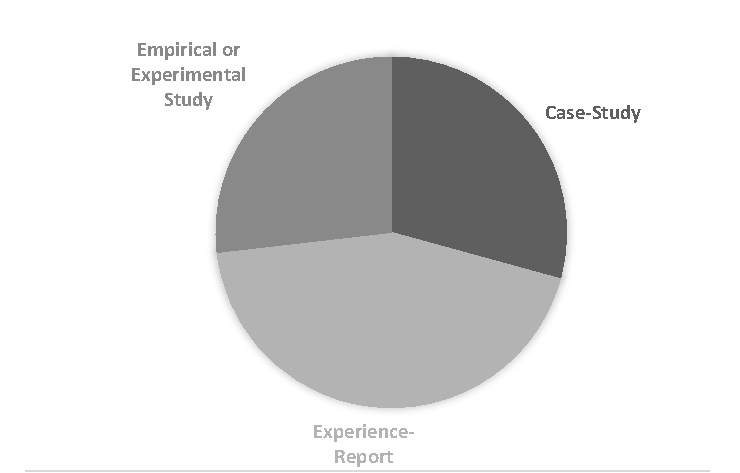
\includegraphics[scale=0.75]{./img/gtypeeval.pdf}
\end{center}
\caption{types of evaluation involved in the grey-literature; experience reports are the striking majority.}\label{g3}
\end{figure}

On the white-literature front, Fig. \ref{w1} offers an overview of the types of studies reported in literature, with a majority of case-studies being targeted for further research.

\begin{figure}
\begin{center}
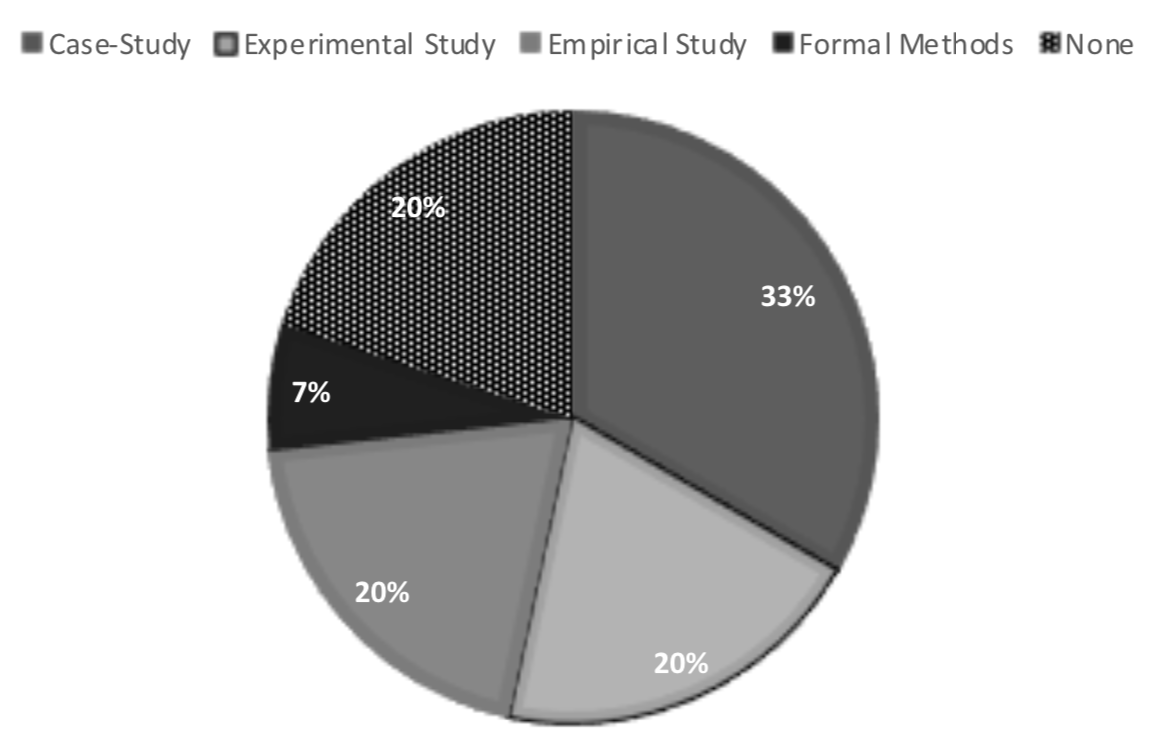
\includegraphics[scale=0.5]{./img/weval.png}
\end{center}
\caption{types of studies conducted in white-literature; case-studies are targeted the most.}\label{w1}
\end{figure}

Beyond the types of studies, Figures \ref{w2} to \ref{w3} offer an overview of the topic interest --- which reflects some mixed trends --- and the typical venues, with a striking preference for conferences --- which are typically more divulgative in nature.

\begin{figure}
\begin{center}
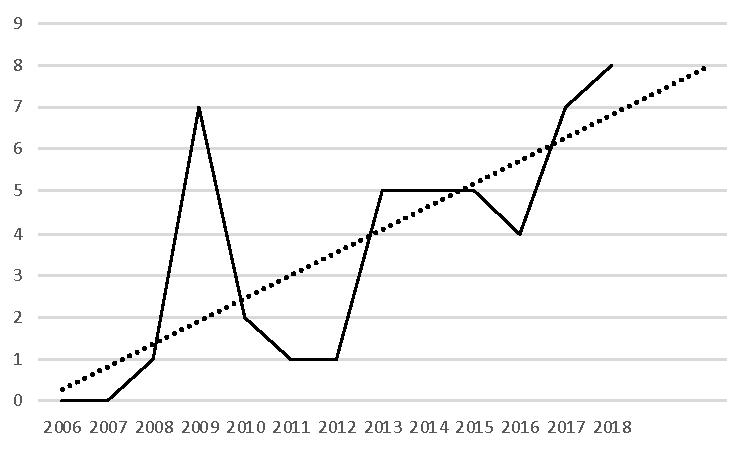
\includegraphics[scale=0.6]{./img/wtimeline.pdf}
\end{center}
\caption{a linear trend is present in white-literature as well; however, mixed but rising interest is reported over the years.}\label{w2}
\end{figure}

\begin{figure}
\begin{center}
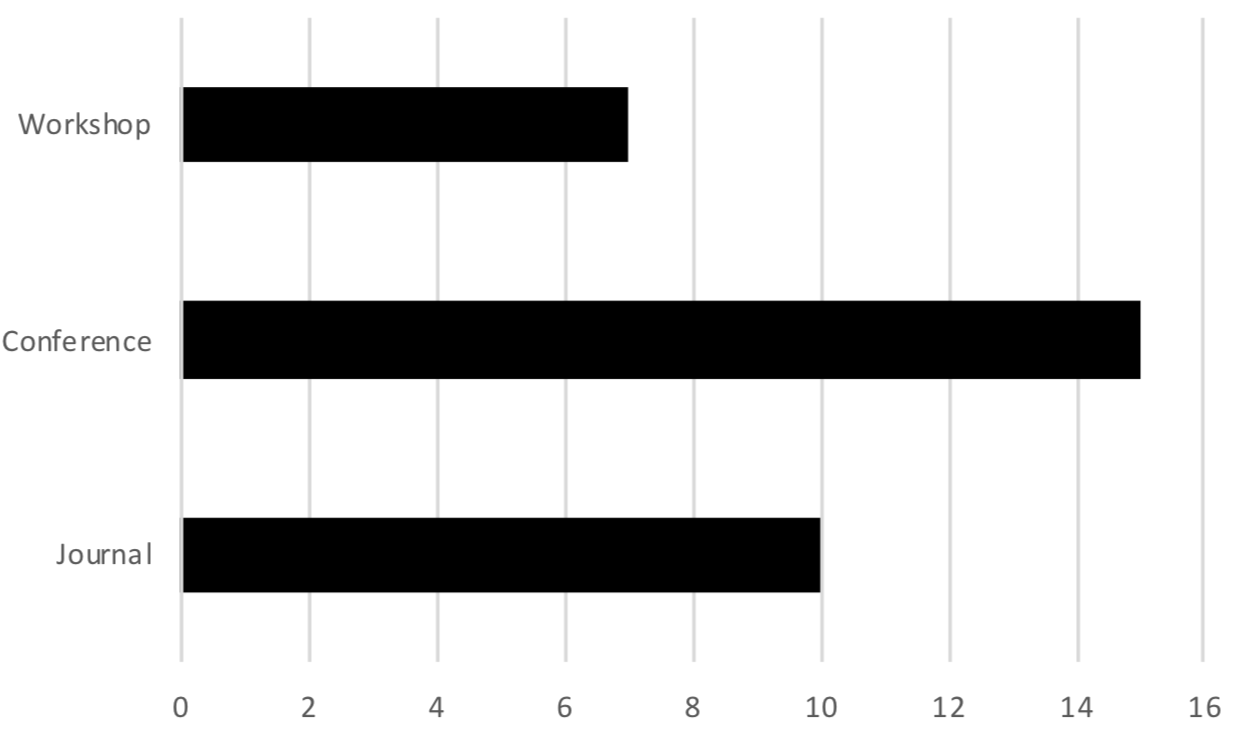
\includegraphics[scale=0.4]{./img/wvenue.png}
\end{center}
\caption{venues selected for publication; the strong preference for conferences or workshops as opposed to journals reflect an emerging discipline.}\label{w3}
\end{figure}

Overall, the statistics offer a not-so-comforting picture. The field seems in an emerging phase, with mixed-feelings or forming interest, typically disseminated in conferences but discussed over case-studies (in white) and/or from experience reports (in grey literature). 

Finally, as an overview of the thematic coding that we adopted to elicit answers for our research questions, Fig. \ref{codescount} offers a quantitative overview of the core concepts discovered as part of our analysis (Definition of codes is provided). The figure highlights that most of the literature we analysed focuses on discussing specific detection \emph{methods} for \emph{criminal activity types}, as opposed to providing holistic methods for the discovery of cybercrime. Moreover, from a quantitative perspective, we highlight that  \emph{website appearance} and their degree of (software) \emph{security} are major indicators for risk assessment. The next sections offer more detail on the results of our study.

\begin{figure}
\begin{center}
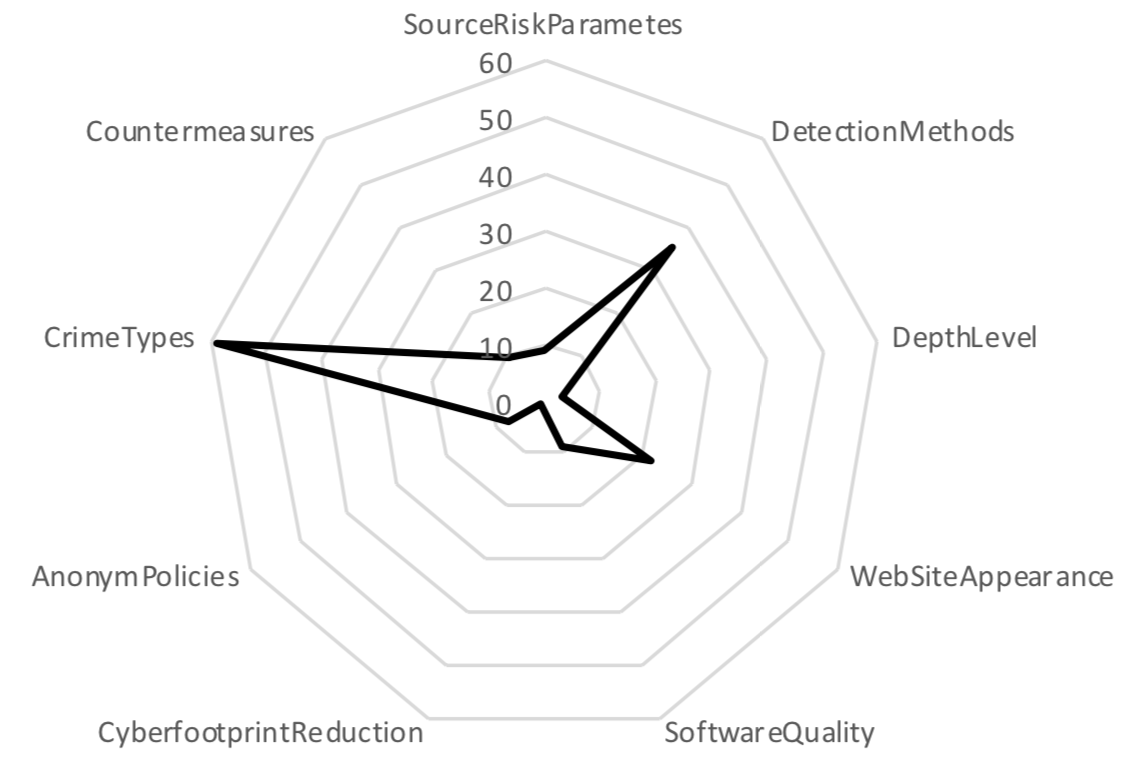
\includegraphics[scale=0.4]{codescount.png}
\end{center}
\caption{Count of occurrences for core-concepts across our dataset, normalized on a percentile scale.}\label{codescount}
\end{figure}

\subsection{Cybercrime Threat Intelligence: A Surface-Web Taxonomy}

Figure \ref{taxo1} outlines the result of our thematic coding as applied to literature discussing or targeting analyses on the \emph{surface} web only.

\begin{figure}
\begin{center}
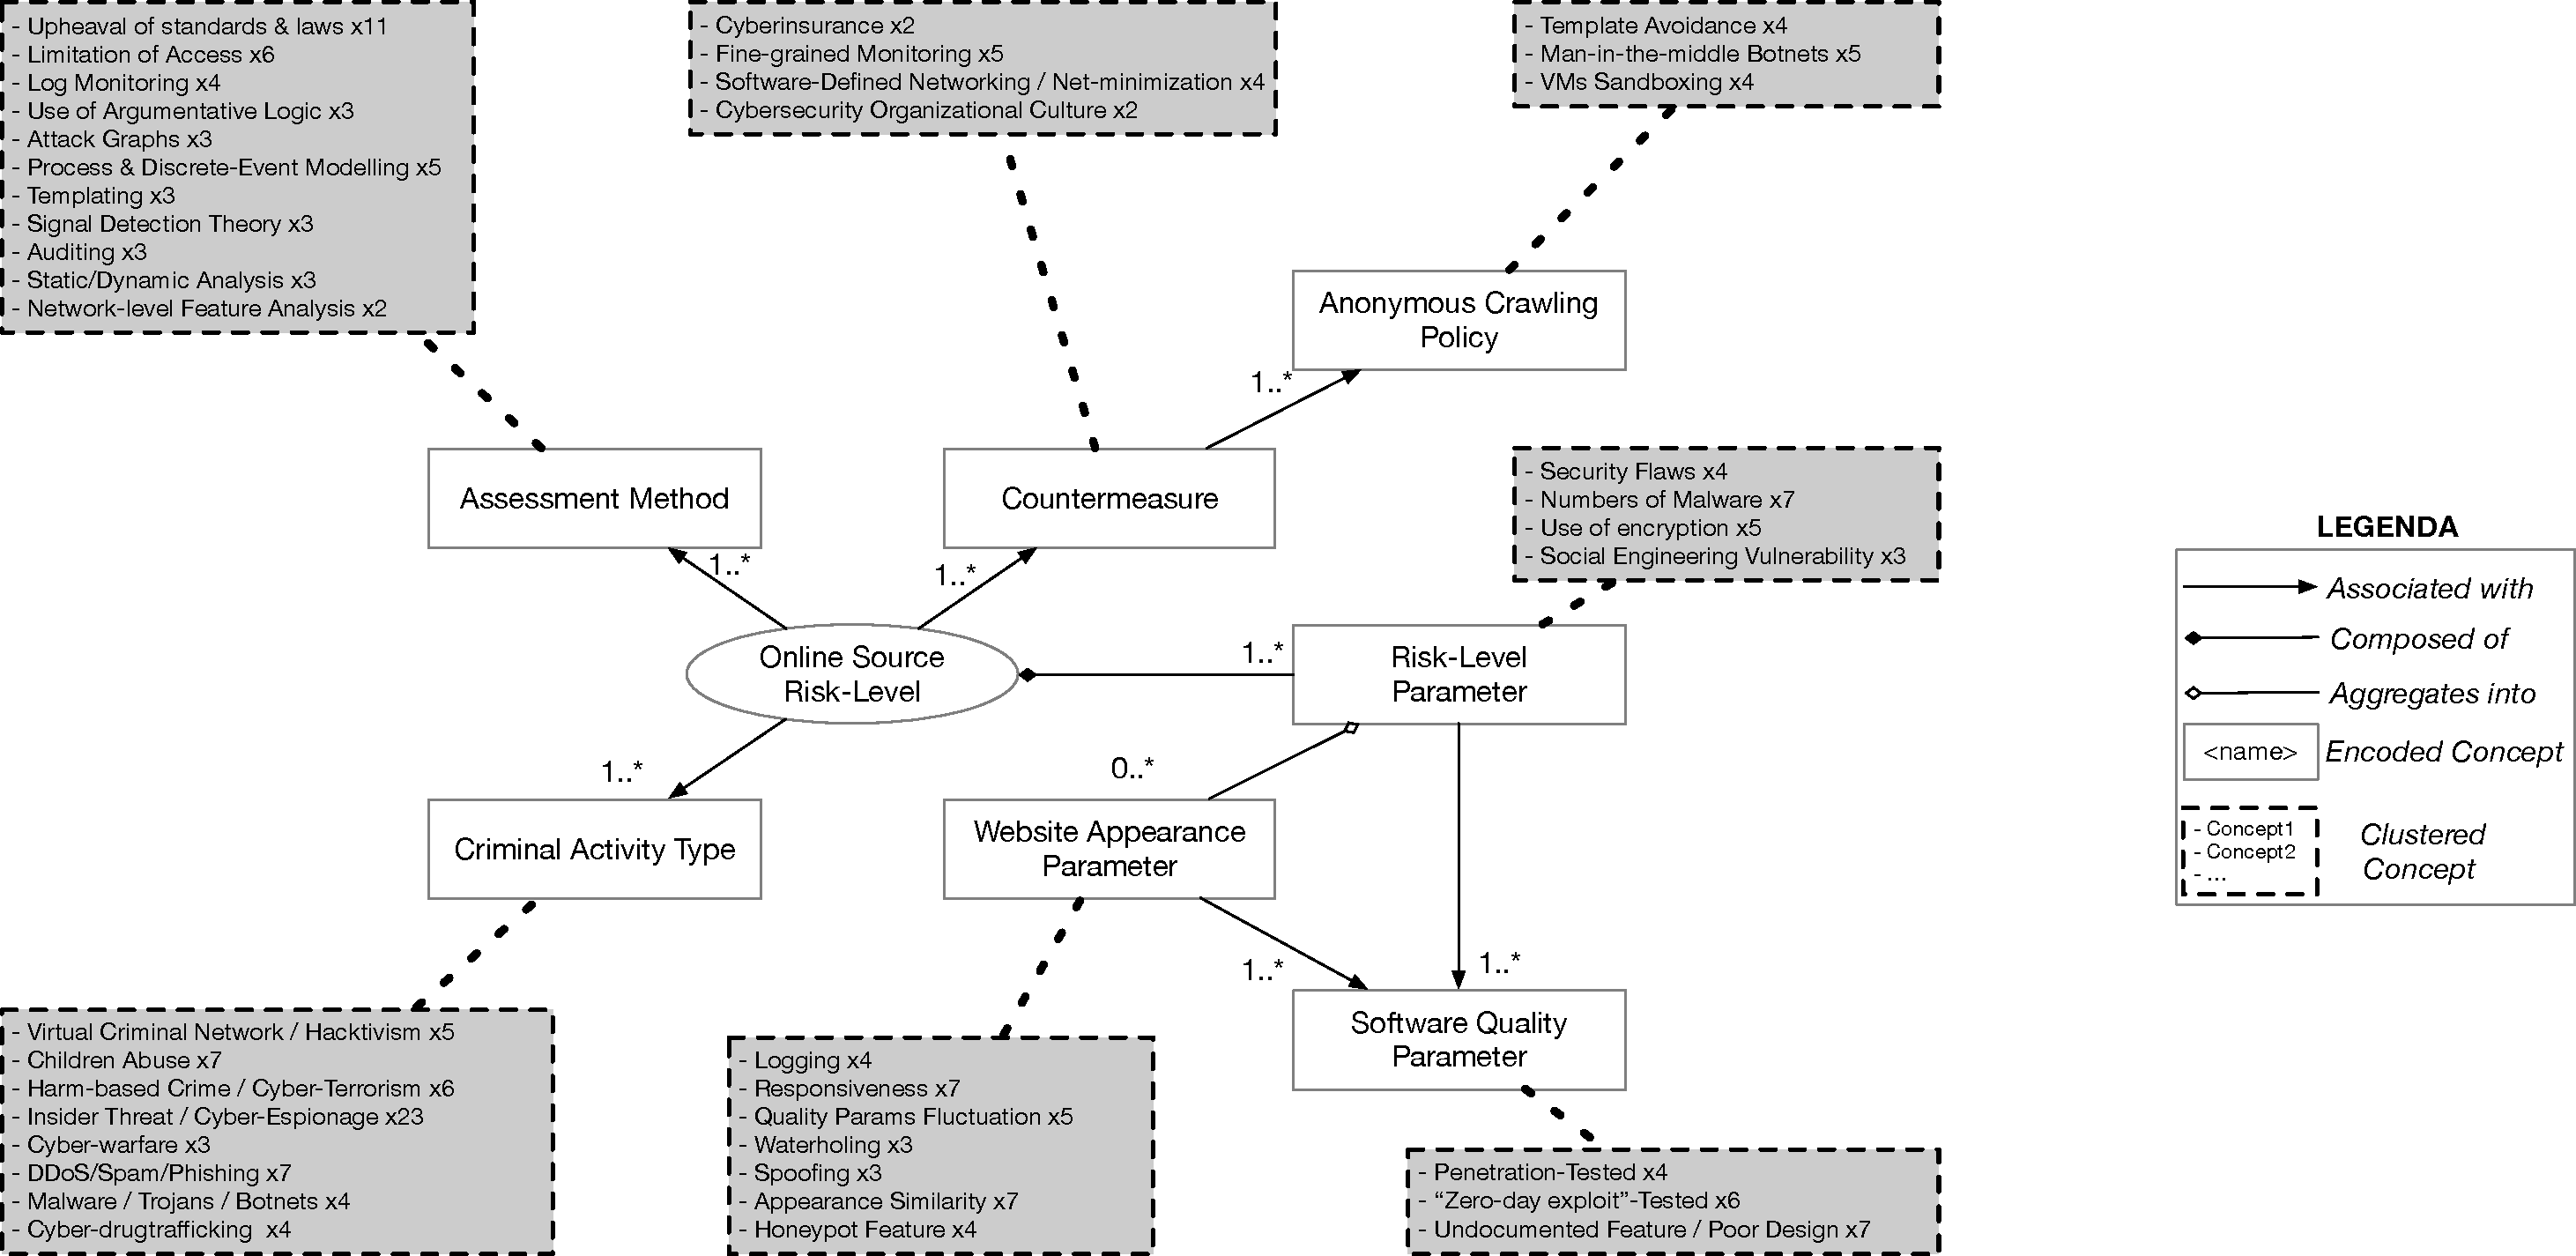
\includegraphics[scale=0.3]{./img/taxo1.pdf}
\end{center}
\caption{A taxonomy of cybercrime threat intelligence for the surface web.}\label{taxo1}
\end{figure}



The results are articulated using a simple UML-like model structured using the core-concepts (inner-most, white boxes on Fig. \ref{taxo1}) emerging from our thematic coding, namely: (a) \emph{assessment methods} --- these are the methods, techniques or tools discussed in the state of the art to address cybercrime threat intelligence; (b) \emph{countermeasures} --- these are the methods and measures that can limit the damage connected to cybercrime, as discussed in literature; (c) \emph{anonymous crawling policy} --- these are the techniques and policies that can limit the detection risk of conducting cybercrime threat intelligence in the open; (d) \emph{risk-level parameters} --- these are indicators for increased risk of specific cybercrimes; (e) \emph{web-site appearance parameters} --- these are ``hints" that previous research identifies as a certain factor indicating that a web source is hosting a specific criminal activity; (f) \emph{software-quality parameter} --- these are software-related quality metrics (e.g., increased throughput or reduced responsiveness) that indicate or are connected to a specific criminal activity being perpetrated; (g) \emph{criminal activity type} --- these are the actual criminal activities being carried out.

The outer-most, grey-colored boxes on Fig. \ref{taxo1} outline what we reported from literature, with a frequency cut-off of 3 recurrences over 3 primary studies from *both* grey and white literature, meaning that concepts, techniques, tools and methods discussed less than 3 times and published or discussed before 2018 were not reported for the sake of space. 

In the following, we flesh-out the results from Fig. \ref{taxo1} in the same order as the core-concepts were outlined in the text above; resulting concepts appear in \emph{italics} in the descriptive sections. It should be noted that, from this point forward, no distinction is made between grey or white literature to avoid any bias in the exposition of the results.

\subsubsection{Assessment Methods}

From a policy perspective, literature remarks that the use of \emph{standards and laws} is the single most-used risk assessment method against cybercrime activity; for example, several articles in both grey and white literature remark that the Gramm-Leach-Bliley Act (GLBA) \cite{Chen2004c} or the Fair Credit Reporting Act (FCRA) \cite{Hoofnagle2013} offer the technical and legal basis to establish the perpetration of online financial crimes of multiple types. In over 30\% of our sample, similar legislations (including GDPR in more modern instances) are suggested as tools in their own right to be used against cybercrime of a more shallow and evident nature in the surface web. Furthermore, several experience reports and case-studies elaborate on the use of \emph{limitation of access} or access-control blacklists as a method to establish and limit the involvement with cybercrime. More specifically, tools and approaches such as SquidGuard~\footnote{\url{http://squidguard.mesd.k12.or.us/}} offer a basis to share and adopt lists of sites hosting criminal activities to be avoided. 

From a more technical perspective, \emph{log monitoring} is highlighted as the most obvious cybercrime risk detection and avoidance method. For example, Mataracioglu et al. \cite{MataraciogluOH15} report on a cybercrime and cybersecurity framework which harnesses log monitoring to detect and avoid social engineering tactics often employed as part of cybercrime. A similar argument is made for the use of log monitoring in several articles from the proceedings of the federated conference on Data Privacy Management, Autonomous Spontaneous Security, and Security Assurance \cite{2014-8872}. In  these venues, log monitoring is combined with \emph{attack graphs}, a formalism built on top of log monitoring techniques that can elicit social engineering attacks by dissecting the connected social engineering threats and vulnerabilities \cite{BeckersKY14}. Similarly to attack graphs, log monitoring and similar runtime threat detection and avoidance activities combine \emph{process modelling/mining} and \emph{argumentative logic}. For example, Bouyahia et al. \cite{BouyahiaICCA14} introduce a metrics-based technique to assist the detection and avoidance of security threats using reasoning systems which incrementally figure out ongoing attacks --- while ontology-based approaches are highlighted in the paper, the authors also remark on the potential to combine a more data-driven machine-intelligence approach. 



From a process mining and modelling perspective, the techniques of \emph{discrete event modelling} dating back to '97 and to Harel and Gery seminal work on object state charts \cite{HarelGery1997}, to signals-detection theory \cite{Green1989} and signals intelligence \cite{MaLPLWZL18} applied to \emph{static/dynamic networks traffic analysis}, and ending up with a recent work focusing on terrorist attacks by Gabriels et al. \cite{abrielSBSGM17}.

Overall, on the one hand, the state of the art results as *very* domain-specific (e.g., terrorist attacks \cite{abrielSBSGM17}, insider threats \cite{Blackwell2009}) mostly based on \emph{templating} of crimes --- that is, offering a standardized format for the perpetrated crime and matching that format onto available data --- and with little generalizable approaches. 

On the other hand, the last two approaches we reported as recurrent, namely, \emph{auditing} and \emph{network-level feature analysis} offer theoretical bases for generalisability. More specifically, cybercrime auditing entails providing for strategic checking of organisational and technical infrastructures by randomly selecting a cybercrime type, instrumenting the type and purposefully targeting the organisational and technical infrastructures with it to evaluate the target infrastructures' vulnerability to it~\footnote{\url{http://m.isaca.org/knowledge-center/research/researchdeliverables/pages/cybercrime-audit-assurance-program.aspx}}. With respect to the auditing technicque highlighted above, Chang et al. \cite{ChangVWL13} offer an in-depth overview of malware-based crimes which is offered as a basis for targeted auditing.

Finally, with respect to network traffic analysis, several approaches reported in literature offer feature-based (social) network analysis \cite{ORiordanFN16} as well as feature engineering and analysis techniques aimed at establishing precursors of social engineering, most notably from our dataset the works by Vidal et al. \cite{VidalC17} or Garibi et al. \cite{abs-1201-0949}.

\subsubsection{Countermeasures}

As previously specified, with the term \emph{countermeasure} we identify the ability to foresee and enact preemptive or corrective action against a specific cybercriminal activity. On one hand, most of the grey literature highlights the need to conduct business-level impact assessment and incident management, for example, the report of the Australian Government \cite{ring2017data} remarks that businesses need to be arrange, quoting from the original document, specific \emph{``actions taken as soon as an attack or breach has occurred to determine the (1) depth of its effect on the business, (2) your ability to recover, and (3) affect the likelihood of future breaches"}. Several proactive actions have been introduced. For example, Baer et al. discuss several approaches to Cyberinsurance \cite{BaerP07} and similarly, earlier works by Meland et al. \cite{MelandTS15} establish the ways in which cyberinsurance actions can be planned as part of corporate governance and towards the reduction of cyberthreats risks.

From a more analytical perspective, several technical countermeasures were proposed, mostly along the lines of fine-grained monitoring of IT assets and business processing; more specifically
Ma et al \cite{Ma2012}, as early as 2012, offer a ightweight framework for monitoring public clouds which is outlined as a potential solution for mitigating cyberthreats, as long as an appropriate incident response organisational structure and culture \cite{ChangL07,TangLZ16} is also in place whereupon a threat does manifest. Later works offer prototypical solutions where cloud and IT infrastructures monitoring is combined with real-time applications security \cite{CoppolinoDFR14}. Still on a technical perspective, acting as a countermeasure for cybercrime is the use of software-defined networks (SDNs) as well as virtual-networks functions (VNFs), that is, harnesssing with programmable/controllable software the responsibility of handling specific network functions that run on one or more virtual machines. In this specific domain, the survey by Hayward et al. \cite{scotthayward2013sec} offers an overview of the practices in SDNs which can be used to attain software-controlled granular cybersecurity and safety.

\subsubsection{Anonymous Crawling Policies}

In terms of maintaining anonymity while performing cybercrime detection or avoidance tasks across an organizational structure, much research has devoted to the use and refinement of Bots and botnets dedicated to detect social engineering attacks or perform anonymous analysis. For example, the works by Lauinger et al. \cite{LauingerPBK10} and subsequent trials by the US Chamber of commerce contained in their whitepaper\footnote{\url{https://www.uschamber.com/CybersecurityEssentials}} remark that \emph{``an acceptable-use policy for the use of information resources and IT systems [needs] for example, confidential or sensitive business information not to be posted by employees on social networking sites such as Facebook or MySpace [...]"}; the aforementioned actions were experimented upon with the usage of policy-driven bots to perform counterinsurgency of amended actions. Likewise the survey by Chang et al. \cite{ChangVWL13} offers an overview of several approaches along the lines defined above wherefore web-based malware is detected, risk-assessed, avoided using on-purpose, policy-driven botnets. 

Finally, in terms of anonymity during detection phases for cybercriminal activity, the use of Virtual-Machine sandboxes is often referred to as the only viable mechanism \cite{ChangVWL13} but several recent works show the endurance of specific attacks or other masqueraded cybecriminal activity such as the S\$A and similar shared-cache attacks \cite{ApececheaES15} against a sandboxing approach.

\subsubsection{Risk-Level Parameters}

This section showcases the few parameters reported in literature which are commonly known to increase the risks of cybercriminal activity being perpetrated in targeted online sources. An outstanding number of whitepapers and governmental reports highlight the presence and proliferation of several risk-related parameters; most notably, as noted in the US Chamber of commerce whitepaper about cybercrime\footnote{\url{https://www.uschamber.com/CybersecurityEssentials}}, ``[actions need to be taken to] root out security flaws in computer programs and to counter cyberattacks by ``bad" hackers, or cybercriminals", hence indicating the presence and extent of security flaws (of which, the number of Malware is an established minimum, as noted by Rahul et al. \cite{Rahul} and several others \cite{Caballero12}) in the code of online sites as a probable factor of risk in establishing high-threat sources. Finally, the haphazard use (or lack thereof) of encryption across online source functions has been established to lead to cybercriminal activity, most notably in the roadmap defined by Kieseberg et al. \cite{KiesebergSR15}. More specifically, the lack of encryption is often connected to the use of specific social engineering activities being perpetrated in online sources, which themselves are functional to cybercrime \cite{Gharibi}. On this latter front, that of social engineering vulnerabilities specifically designed to accomodate for cybercriminal activity, several authors such as Vidal et al. \cite{VidalC17} remark on the necessity to conduct scenario-based situational crime prevention, e.g., using evolutionary computing and social predictive analytics --- the work along these lines has mostly concentrated on elaborating more or less complete cyberforensics ontologies for the purpose of knowledge representation and reasoning about cybercriminal investigation in a scenario-based fashion \cite{ParkCK09}.

\subsubsection{Software Quality Parameters}

The necessity to establish security as a software quality parameter to decide whether an online source bears risk of cybercriminal activity finds agreement in ~90\% of both grey and white literature alike. More specifically, the quality of software security is established around three axes: (1) whether the online source bear signatures and certificates of successful penetration-testing \cite{franklin}; (2) whether the online source has been certified against morphisms \cite{li06ieee,GuptaR18} of known zero-day exploits \cite{Danforth11,BilgeD13}; (3) finally, whether the online source bears undocumented software features and/or the indications of poor design (e.g., technical debt, etc.) \cite{NordOSSK16}.

\subsubsection{Website-Appearance Parameters}

In terms of website appearance, the literature we analysed identifies seven features as indicative pre-conditions to cybercriminal activity: (1) the lack of logging as well as software features for forward error correction, site responsiveness as well as other constructs that measure all graph-theoretic properties of the darknet (e.g., see Griffith et al. \cite{GriffithXR17}); (2) variable responsiveness rates from the online source \cite{} (3) a heavy fluctuation of the overall software quality parameters (e.g., language clarity, documentation, feature stability, etc.) for the online source, oftentimes detected thorugh anomaly detection or linear-time temporal logics, as seen in Almukaynizi et al. \cite{AlmukayniziPSSS18}; (4) the existence of waterholing features, defined by Trendmico\footnote{\url{https://www.trendmicro.com/vinfo/in/threat-encyclopedia/web-attack/137/watering-hole-101}} as areas of the site which are uncontrolled, uncontrollable, or never improved overtime by site maintainers \cite{KhanIJKBIES}; (5) the presence of spoofed information mismatches detectable through online fact-checking, an approach to this is presented in Nunes et al. \cite{NunesSS18}; (6) a high degree of appearance similarity with respect to other known online sources \cite{GhoshPYND17,MartineR05}; (7) finally, honeypot features most predominantly the length and target of the redirection chain upon any navigation request from the source, since almost 68\% of our sources from white and grey literature studies observe that malicious landing sites almost always have unusually long redirection chains toward malware distribution sites \cite{ChangVWL13}.

\subsubsection{Criminal Activity Types}

Lastly, the risk assessment of online sources can be supported by focusing the identification of the risk using combined measures of likelihood for reported criminal activity types \cite{Elstob74}. This section outlines and discusses all criminal activity types we reported in literature. As previously remarked, we report in this section the crime types reported at least 3 times in at least 3 papers from both grey and white literature (i.e., at least 6 papers in total), later in Sec. \ref{disc} we discuss emerging crime activity types reported in more recent literature. Overall, the literature on cyberthreat intelligence focuses around 7 criminal activity types, namely: (1) Virtual Criminal Network / Hacktivism Groups --- these reflect, on the one hand, crime networks dedicated to regular crime activity (e.g., drug trafficking) exploiting online means \cite{HanWCMZ17} and, on the other hand, forms of cyber-activism (i.e., Hacktivism), where cyber attacks are ideologically motivated and have primarily a demonstrative intent, like damaging the image of the target and/or causing a temporary malfunctioning of the attacked ICT systems \cite{sureka2010mining}; (2) Children Abuse --- these reflect sites exploiting minors for malicious intents and purposes, including and not limited to humans trafficking \cite{HanWCMZ17}; (3) Harm-based Crime / Cyber-Terrorism --- these activities are usually ideologically motivated, as outlined by Gordon \cite{GordonF02}, and uses exploitations of systems vulnerabilities with the intent of influencing a state or an international organization \cite{VeerasamyG15};  (4) Insider Threat / Cyber-Espionage --- these activities focus on the exploitation of organizational insiders \cite{Rocha15a} for the purpose of information trafficking and intelligence, with works ranging from classification of threat intelligence risks \cite{SantosNYKLWOJC12} to stream reasoning technology for live detection of leaks \cite{ParveenMWETHK13}. Oftentimes such cyber-espionage is functional to (5) Cyber-warfare --- these activities focus on operations carried out in the cyber domain with the purpose of achieving an operational advantage of military significance, with a full report from the US Military intelligence \cite{Cordesman2002} as a seminal work; (6) DDoS/Spam/Phishing --- similarly to cyber-espionage Distributed Denial of Service \cite{Kandula05}, Spam or Phishing criminal activities are connected to crimes against critical infrastructures \cite{setola2016critical} - for example attacks affecting the integrity of data or information systems used in Supervisory Control and Data Acquisition Systems (SCADA) could be used to overload power grids, block communications and financial transfers, etc; (7) cyber drug-trafficking --- these activities focus on the stockade, movement, production, and reselling of illegal substances, wit early works focusing on identifying the extent and properties of the collaboration networks lying beneath \cite{Wood17}.

Overall for the above crimes all have been reported in connection to software-based electronic threats, vulnerabilities, and attacks where Malware (including ransomware and similar malware aiming explicitly at financial gains), Trojans, or Botnets play an instrumental knowledge-gathering and insurgency role, with latest works on this research stream discussing the architectural properties of malware altogether, e.g., Lakhotia et al. \cite{LakhotiaB17}.


\subsection{Cybercrime Threat Intelligence: A Taxonomy for Deep- and Dark-Web}

Beyond the previously defined taxonomy addressing the surface web, this section discusses the approaches, countermeasures, indicators for Cybercrime Threat Intelligence in the deep- and dark-webs. The taxonomy in question (see Fig. \ref{taxo2}) shares overlaps with its surface web counterpart (see Fig. \ref{taxo1}), specifically in the criminal activity types and countermeasures thereof (see the greyed boxes with ``.*" symbol).

\begin{figure}
\begin{center}
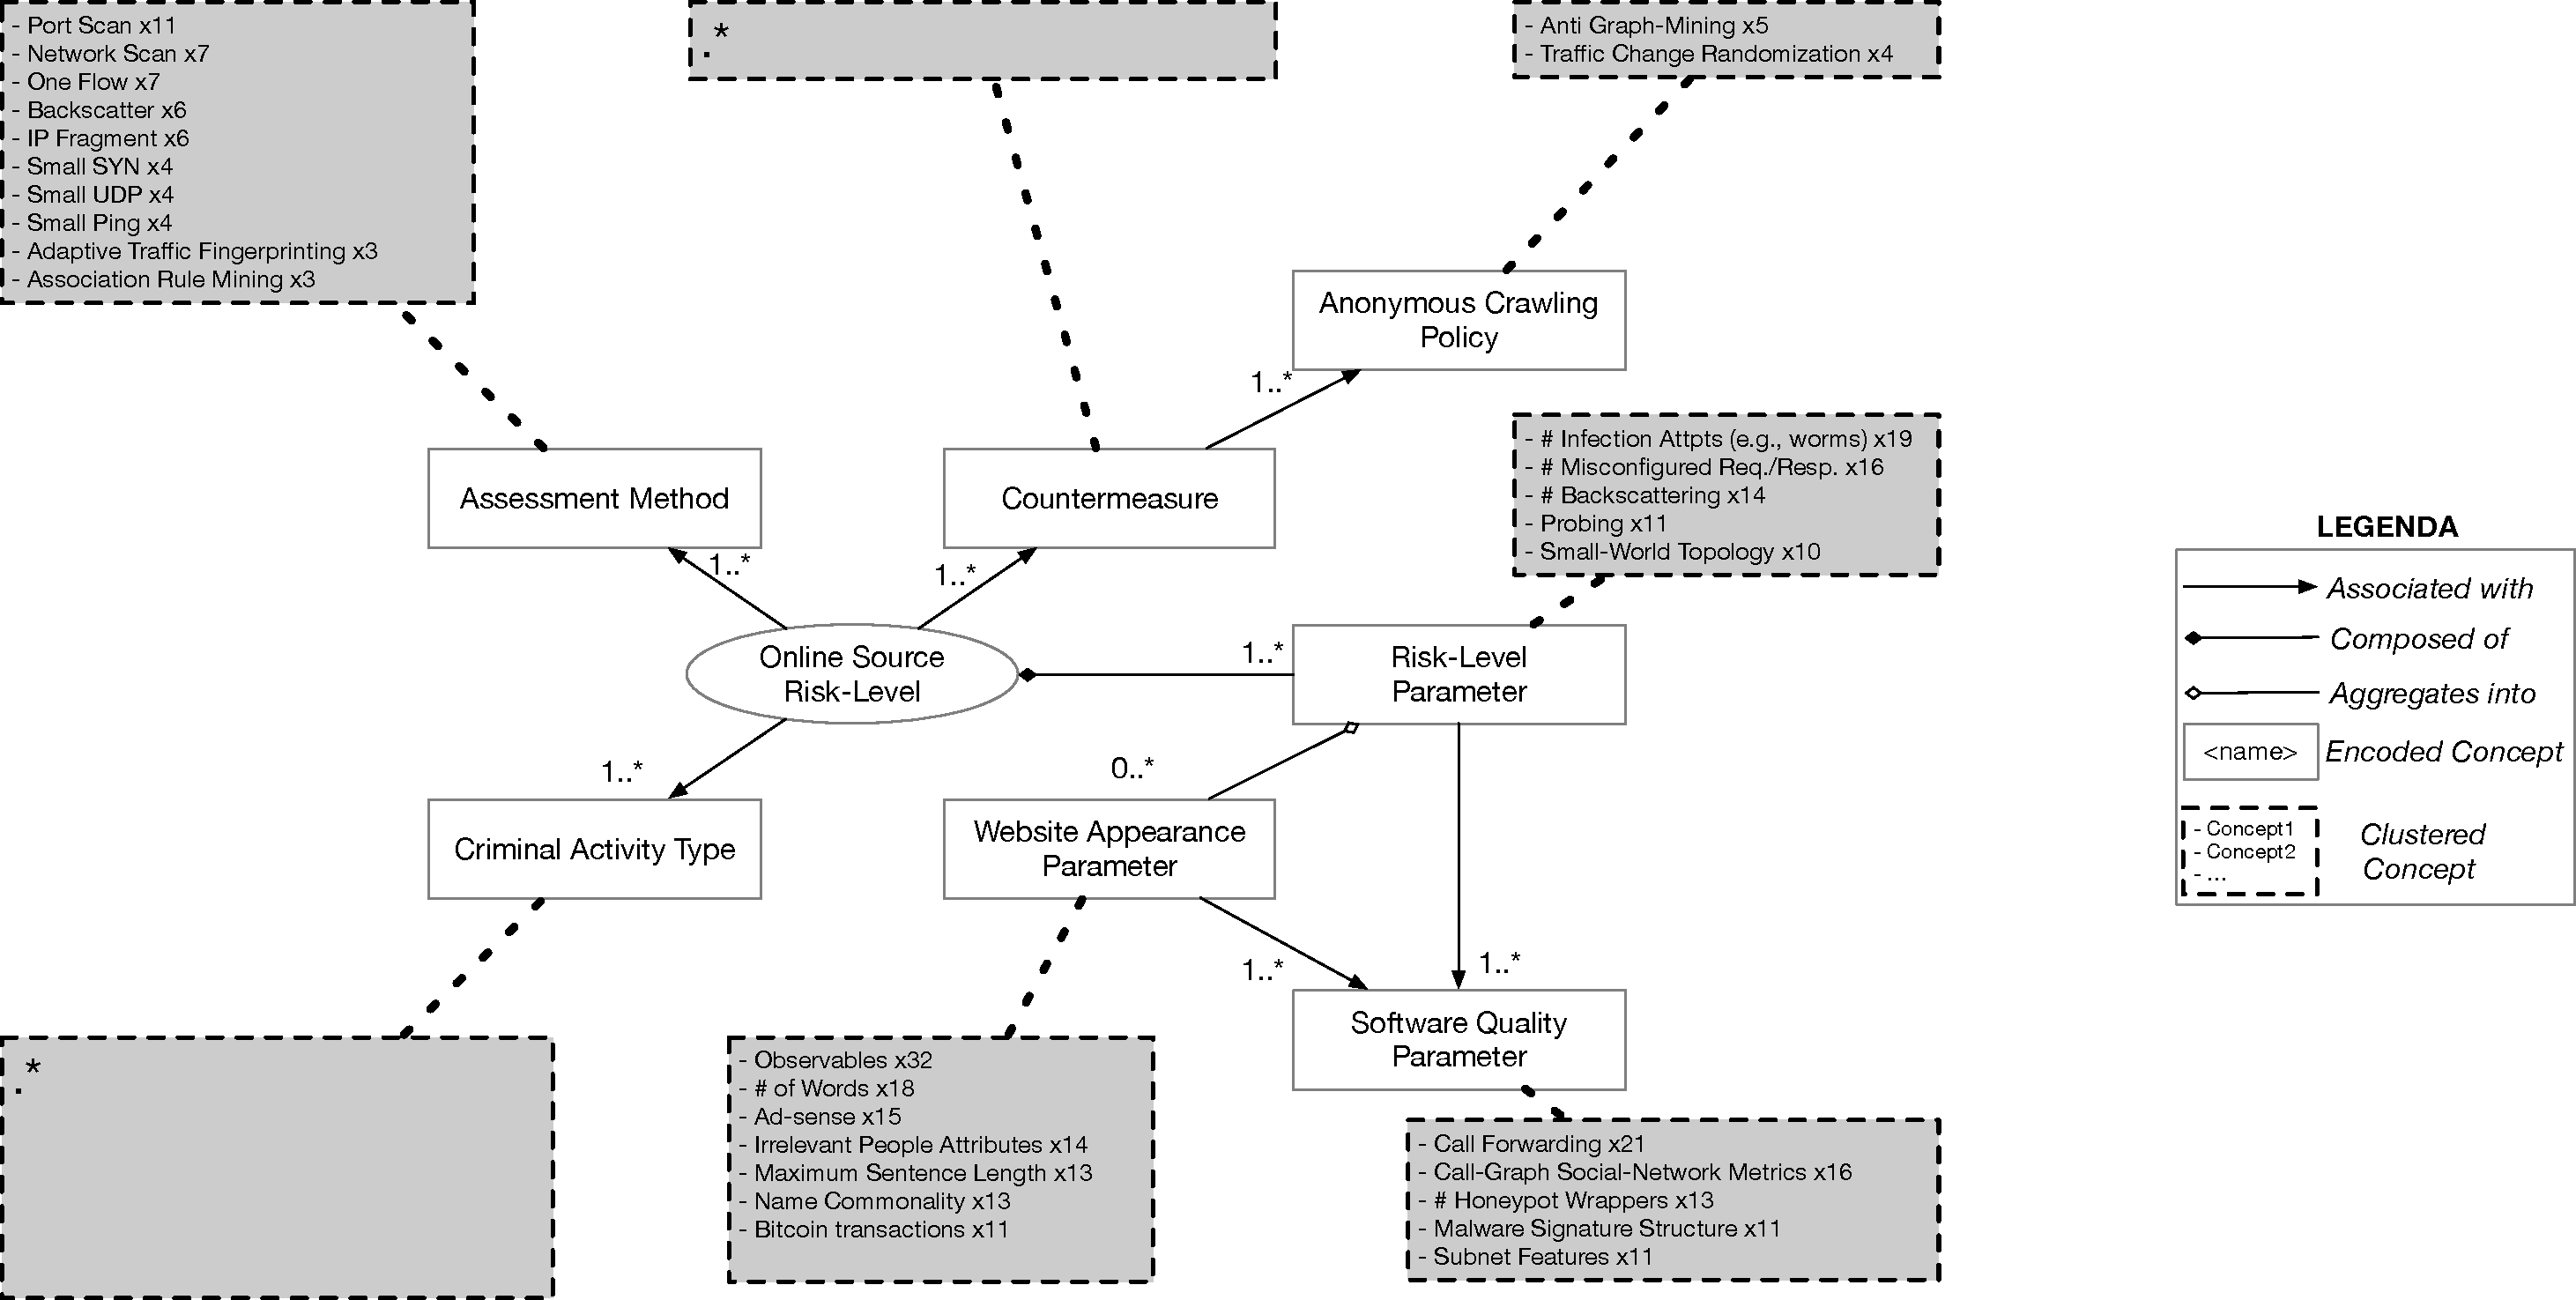
\includegraphics[scale=0.3]{./img/taxo2.pdf}
\end{center}
\caption{A taxonomy of cybercrime threat intelligence for the surface web.}\label{taxo2}
\end{figure}

\subsubsection{Assessment Methods}

The assessment methods harnessed for the investigation in the context of deep-web and darknets are considerably different with respect to their surface internet counterparts. Data indicates a distinct use of port-scan \cite{GadgeP08,KikuchiFTD08} techniques as a basis for assessment, namely, detecting port activity in or around a specific host. Most recent works along these lines reported in our dataset is from Neu et al. \cite{NeuTLMOZ18} offer glimpse of port-scan technology in the context of Software-Defined Networks (SDNs) \cite{sorensen2012} as well as Ring et al. \cite{ring2018} who manage to detect port-scans at large-scale; a similar attempt to Ring et al. comes from Affinito et al. \cite{Affinito2018} who implement a stream analysis campaign over Apache Spark to instrument for large-scale port-scans. From a higher level of abstraction, network scans \cite{MazelFF16} are reported as the second most-frequent method for online source risk assessment; network scans are defined as a procedure for identifying active hosts on a network, either for the purpose of attacking them or for network security assessment \cite{LeckieR02}. Recent research in this domain shares the same aims as port-scanning research, i.e., detection and avoidance. Concerning the remainder of the approaches, a very valuable recap is offered by Liu et al. \cite{LiuF18}. More specifically, OneFlow analysis concerns analysis of large-scale traffic directed at single entry-points inside a network \cite{YegneswaranBP04,NishikazeOKBNS15} while Backscattering \cite{BalkanliZH15} and IP-Fragment analysis \cite{KimKH13} concern identifying different aspects of DDoS attacks, namely, response packets to (D)DoS attacks carried out elsewhere in the Internet and attempts to defeat packet filter policies. Furthermore, small-* analysis techniques aim at establishing anomalies in network traffic reflecting a minimum amount of specific packet types (e.g., SYN, UDP, Ping) --- a very valuable comparative outline of these approaches is contained in Kumar et al. \cite{kumar2014intrusion}.

\subsubsection{Anonymous Crawling Policies}

Considering the invasiveness of assessment methods, we were not surprised not to find many approaches to anonymous crawling and cybercriminal activity assessment. The few literature elements that do exist discuss the use of countermeasures to graph-mining \cite{PhillipsL09} as mechanisms to prevent detection of cybercriminal activity assessment, e.g., by rearranging network topologies by means of software-defined networking. Similarly, Haughey et al. provide evidence for use of traffic randomization  to avoid adaptive traffic fingerprinting \cite{Haughey18}.

\subsubsection{Risk-Level Parameters}

Risk-level parameters offered by literature in threat intelligence range from infection attempts coming from a specific source \cite{Yannikos2018} as well as misconfigured request-response messaging patterns \cite{7317717}; in this context, the recurrent use of backscattering counts from specific sites has been reported as indicative of high-risk online sources \cite{Fachkha16}. Likewise, the number of probe code instances, that is, code designed to attempt gaining access to a networked host and its files through a known or probable weak point, has been established as a proxy for high-risk online sources \cite{CanepaC13}. Finally, risk analysts can use an assessment of a small-world topology condition reflecting the links and call-forwarding structure stemming from the source \cite{Narayanan2009,Kleinberg2000}.

\subsubsection{Software Quality Parameters}

In terms of software quality characteristics that can be used as proxy for cybercriminal activity, the literature is again not conclusive. 
On one hand, the use of graph-based intelligence includes parameters such as call-forwarding occurrences \cite{Huang2018} in the online source code as well as inferential social-networks metrics applied to call-forward graphs \cite{Monk18}. On the other hand, related literature in malware detection and avoidance suggests the study of malware code (e.g., counting honeypot wrappers \cite{Schneider2011Mitigation,Bou-HarbDA15}) to identify signature structures matching specific cybercrime \cite{ShoshaLGM12} as well as studying the subnetting structure in a call-forward graph and the hosts therein \cite{abs-1811-10050,AhrendJJ16}.

\subsubsection{Website-Appearance Parameters}

Finally, in terms of the appearance of online sources, several parameters emerged which are germane to establishing the cybercrime risks for such online sources. Most specifically, the amount of observable (i.e., monitorable and loggable) characteristics, or \emph{observables} \cite{NabkiFAP17} of the source along with the number of words employed for textual descriptions as well as typical name commonalities \cite{} around the source \cite{SkopikSF16,NaritaKOBT16}; individual characteristics of words and phrases (e.g., as reflected by Maximum Sentence Length \cite{Bailey2006PracticalDM}) are also suggested as indicative \cite{YangSZW07}. Beyond simplistic counts, related literature on website-appearance from deep- and darknets highlights the use of ad-sense as well as irrelevant people attributes \cite{WangWSTGCJ18} being requested for registration as primary indicators of specific cybercriminal activities \cite{YangSZW07}. For example, specific people attributes (e.g., bitcoin accounts and transactions thereof \cite{Khelghati16}) are often associate to illegal-trafficking.

\subsection{Cybercrime Threat Indicators: Topic Modelling Results}

In this paragraph we are now going to discuss the results of our Topic Modelling Analysis on our set of papers. As previously stated, we used Latent Dirichlet Allocation (LDA) to highlight the most relevant themes in our textual data, however before applying LDA we pre-processed our text. The pre-processing phase aims at improve our final results and consist of: \emph{i} removal of unwanted chars, numbers and symbols (like words smaller than two chars), \emph{ii} removal of stop-wars, \emph{iii} lemmatization in order to reduce any given word to its root form thereby reducing multiple forms of a word to a single word.
After the pre-processing phase we apply LDA method for visualizing and interpreting topics, the method we used is the one described in \cite{W14-3110} called \textbf{LDAvis} and based on the work of Chuang et. al in \cite{Chuang:2012:TVT:2254556.2254572}. The paper, moreover, gives the instructions to read the diagrams we plotted, however, below continue with a small recap about how to interpret our diagrams. 
On the left side of our figures we have a recap of our topics, each of the circle represent a topic and how prevalent it is, moreover if the circles are overlapping each other means that those topics have common terms. Into each of this circle are sorted our terms in a decreasing order of prevalence.
The right panel of our results depicts a horizontal barchart whose bars represent the individual terms that are the most useful for interpreting the currently selected topic on the left. The overlaid bars represent both the corpus-wide frequency of a given term as well as the topic-specific frequency of the term \cite{W14-3110, Chuang:2012:TVT:2254556.2254572}. The $\lambda$ slider allows to rank the terms according to term relevance. Moving the slider allows to adjust the rank of terms based on much discriminatory (or ``relevant'') are for the specific topic, we fixed the $\lambda$ at 0.8.\todo{suggested value is 0.6, however nothing change with the results}

Here below we are now going to discuss our results of our topic modelling analysis. For each analysis in Fig.~\ref{fig:topicmodelling_1}, Fig.~\ref{fig:topicmodelling_2}~and Fig.~\ref{fig:topicmodelling_3} \todo{missed dark and deep web analysis} we build a table where we summarize and discuss the most relevant terms related to the cybersecurity field. 

\subsubsection{Topic modelling results for Surface Web}

In Table~\ref{tab:topicmodelling_1} we have the list of words from \textit{Topic~1}. 


%%%%%%%%%% TABLE topic 1 %%%%%%%%%%%%%%

\begin{table}[H!]
%\small
%\resizebox{\textwidth}{!}{%
\scalebox{0.8}{
\begin{tabular}{@{}lll@{}}
%\begin{tabular}{p{0.12\textwidth}p{0.8\textwidth}p{0\textwidth}}
\toprule
\textbf{Terms} & \textbf{Score} & \textbf{} \\ \midrule 
\rowcolor[HTML]{EFEFEF} 
System & 40 & \begin{tabular}[c]{@{}l@{}}
The system can receive different type of attacks. The operating system of a PC, if not properly\\ maintained, can easily be the target of virus, worm, malware, spyware and other cyberthreat\\ attacks. In order to protect the system of a private user is important to have an antivirus\\ and keep the system updated. In a private company is important to educate the \\ employee to do not use distrusted applications and to use strong passwords in order to protect\\ personal information. An attack to the system can involve a loss of personal data, a destabilization  \\ of the running processes of the system and the forward of private information to third parties.\end{tabular} \\
\rowcolor[HTML]{FFFFFF} 
Vulnerability & 27 & \begin{tabular}[c]{@{}l@{}} Techopedia defines the therm \textit{vulnerability} as cyber-security term that refers to a flaw in a system\\ that can leave it open to attack. A vulnerability may also refer to any type of weakness in a computer\\ system itself, in a set of procedures, or in anything that leaves information security exposed to a\\ threat \cite{techopedia}. Some computer vulnerabilities include bugs, weak password, outdated operating \\ system, OS command injection, download of pirate software. Computer users and network personnel\\ can protect computer systems from vulnerabilities by keeping software security patches up to date, \\moreover, to better increase our cybersecurity, is important to use programs like firewall, anti-virus,\\ web URL filtering and avoid thye download of pirate software.\end{tabular}\\ 
\rowcolor[HTML]{EFEFEF} 
Threat & 27 & \begin{tabular}[c]{@{}l@{}}  We live in a hyperconnected world, half the world's population is interconnected through Internet\\ and 125 billion of IoT devices are expected by 2030 to be connected. All this complexity along with\\ constantly evolving nature of cybersecurity threats is leading to more breaches and cyber attack\\ threats. Threats are potentials for vulnerabilities to turn into attacks on computer systems, networks,\\ and more. They can put individuals' computer systems and business computers at risk, so\\ vulnerabilities have to be fixed so that attackers cannot infiltrate the system and cause damage.\\ Threats can include everything from viruses, trojans, back doors to outright attacks from hackers \cite{techopedia}.\end{tabular}\\ 
\rowcolor[HTML]{FFFFFF} 
Malware & 17 & \begin{tabular}[c]{@{}l@{}} Malicious software (MALWARE) is one of the most common cyber threat attack. A MALWARE is\\ any software that does harm to the system, such as a virus or spyware. There are a lot of different \\ versions of MALWARE: virus, trojan, rootkit, worm, spyware and adware, all of them with different\\ characteristics but with the same purpose. The aim of all this malicious software is to steal private \\ information from the victim's PC, profile the habits of the victim user, use the attacked machine as a\\ zombie for network attacks.\end{tabular} \\ 
\rowcolor[HTML]{EFEFEF} 
Software & 17 & \begin{tabular}[c]{@{}l@{}} As software prices increase, many users turn to installing bootleg copies, or pirated ones. According \\ to the study in \cite{piracy} 34\% of the downloaded pirated software came bundled with malware that infect\\ the computer once the download is complete or when the folder containing the pirated software is\\ opened. In order to avoid any type of risk, a solution is to use free version of the software or similar\\
software but free or open source. \end{tabular} \\ 
%\rowcolor[HTML]{EFEFEF} 
%Victim & 15 &  \end{tabular}\\ 
\bottomrule
\end{tabular}
}
\caption{Topic analysis results of the first topic in Surface Web.}
\label{tab:topicmodelling_1}
\end{table}




% \begin{table}[h!]
% \small
% \resizebox{\textwidth}{!}{%
% %\begin{tabular}{p{0.10\textwidth}p{0.10\textwidth}p{0.70\textwidth}}
% \begin{tabular}{@{}lll@{}}
% \toprule
% \textbf{Terms} & \textbf{Score} & \textbf{} \\ \midrule 
% \rowcolor[HTML]{EFEFEF}
% Packet & 19 & \begin{tabular}[c]{@{}l@{}} The Denial of Service (DoS) attack is meant to shut down a machine or a network and its services\\ making it inaccessible to the users. The main target of DoS attack are usually  web servers of\\ high-profile organizations such as banking, commerce, and media companies, or government and\\ trade organizations. In general we have two types of DoS attack: flooding services and crashing services.\\ The first is caused by high traffic to the servers that makes the services slow down and eventually stop.\\ In the latter case the DoS attack exploit vulnerabilities in order to let crash the running services or\\ destabilize the system.\end{tabular} \\
% \rowcolor[HTML]{FFFFFF} 
% Website & 19 & \begin{tabular}[c]{@{}l@{}}A website can be the place of cyberthreat attacks if the system behind it is not well updated or if the \\ passwords used by the admin are not strong enough. A compromised website can host different types \\ of cyberthreat attacks. A Phishing website is able to steal passwords and personal information of a \\ user. A website can also be the target of SQL Injection Attack in order to retrieve private information \\ from the database.\end{tabular} \\
% \rowcolor[HTML]{EFEFEF} 
% Network & 13 & \begin{tabular}[c]{@{}l@{}}Network attacks are launched every hour of every day, and they are evolving in complexity and level \\ of danger. WiFi attacks aim at stealing password of a personal network in order to commit illicit actions. \\ The most common attacks to the WiFi network are Fake WiFi Access Points, Evil Twins, and Man in \\ the Middle Attacks all of them in order to intercept the data and steal personal information.\end{tabular} \\
% \rowcolor[HTML]{FFFFFF} 
% Email & 10 & \begin{tabular}[c]{@{}l@{}}The emails are one of the main vehicle of information and data. The Identity Theft attack happen when \\ an attacker is able to gain a handle on the employee's email account. The attacker can then turn into the \\ employee's identity. Phishing Attacks a type of social engineering attack often used to steal user data, \\ including login credentials and credit card numbers. It occurs when an attacker, masquerading as a\\ trusted entity, dupes a victim into opening an email. The recipient is then tricked into clicking a malicious\\ link. Virus as attachment to the email in order to install unwanted software on the PC of the user. Spam\\ email are commonly used in order to deliver Trojan horses, viruses, worms, spyware, and targeted\\ phishing attacks or to bring users on a external website in order to steal private and personal information.\end{tabular} \\
% \rowcolor[HTML]{EFEFEF} 
%  &  &  \\
% \rowcolor[HTML]{EFEFEF} 
%  &  &  \\ \bottomrule
% \end{tabular}
% }
% \caption{Topic analysis results of the first topic in Surface Web.}
% \label{tab:topicmodelling_1}
% \end{table}

%%%%%%%%%%%%%%% ANALIS TOPIC 1

\begin{figure}[H!]
\begin{center}
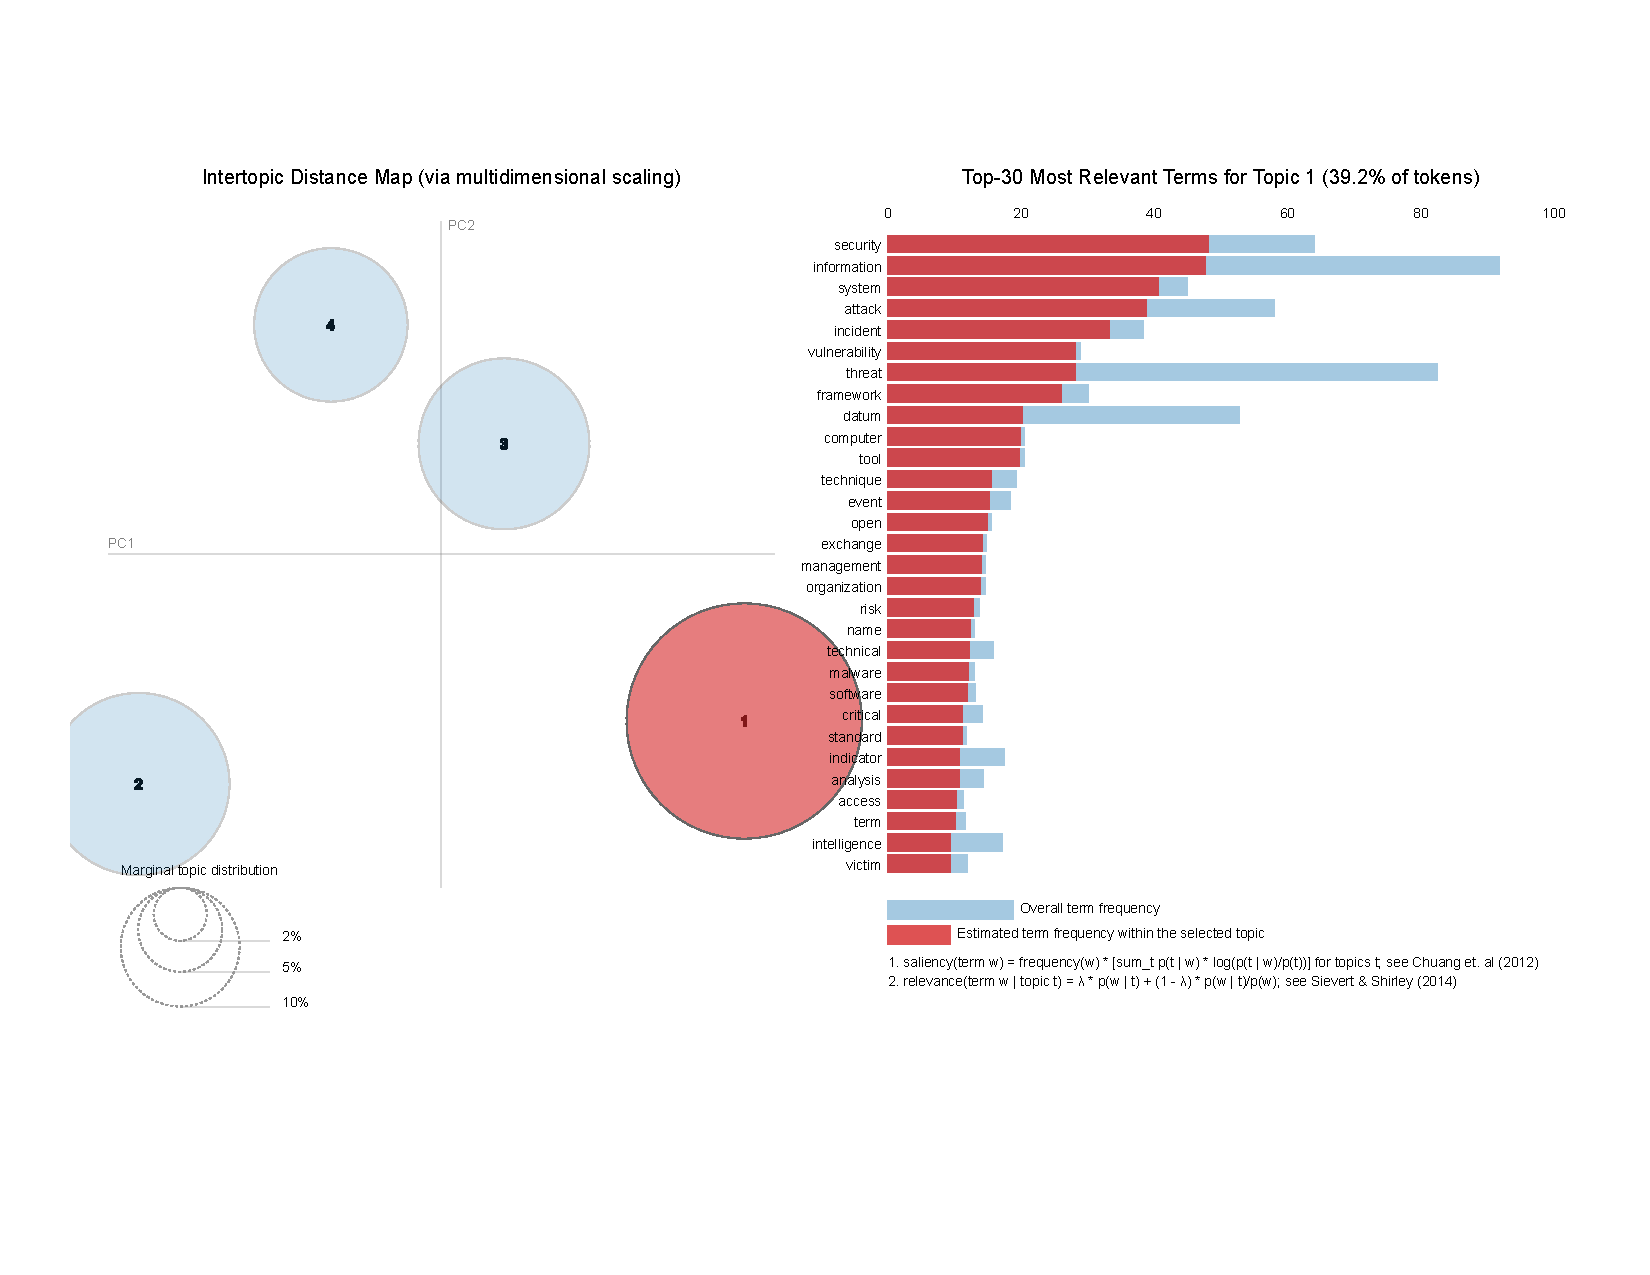
\includegraphics[scale=0.3]{./img/codingALL_topic1.pdf}
\end{center}
\caption{Topic modelling results of the first topic in Surface Web.}
\label{fig:topicmodelling_1}
\end{figure}

%%%%%%%%%%%%%%% %%%%%%%%%%%%%%% 
%%%%%%%%%%%%%%% %%%%%%%%%%%%%%% 
%%%%%%%%%% TABLE topic 2 %%%%%%%%%%%%%%

\begin{table}[h!]
\small
\resizebox{\textwidth}{!}{%
\begin{tabular}{@{}lll@{}}
\toprule
\textbf{Terms} & \textbf{Score} & \textbf{} \\ \midrule 
\rowcolor[HTML]{EFEFEF} 
System & 26 & \begin{tabular}[c]{@{}l@{}}The system can receive different type of attacks. The operating system of a PC, if not properly\\ maintained, can easily be the target of virus, worm, malware, spyware and other cyberthreat\\ attacks. In order to protect the system of a private user is important to have an antivirus\\ and keep the system updated. In a private company is important to educate the \\ employee to do not use distrusted applications and to use strong passwords in order to protect\\ personal information. An attack to the system can involve a loss of personal data, a destabilization  \\ of the running processes of the system and the forward of private information to third parties.\end{tabular} \\
Software & 8 & \begin{tabular}[c]{@{}l@{}}Malicious software (MALWARE) is one of the most common cyber threat attack. A MALWARE is\\ any software that does harm to the system, such as a virus or spyware. There are a lot of different \\ versions of MALWARE: virus, trojan, rootkit, worm, spyware and adware, all of them with different\\ characteristics but with the same purpose. The aim of all this malicious software is to steal private \\ information from the victim's PC, profile the habits of the victim user, use the attacked machine as a\\ zombie for network attacks.\end{tabular} \\
\rowcolor[HTML]{EFEFEF} 
Url & 8 & \begin{tabular}[c]{@{}l@{}}Url is a unique identifier used to locate a resource on the internet. However, often Url's are used to\\ carry unaware users on distrust websites built in order to steal personal information and banking \\ coordinates and passwords. Url's are spread through emails, gaming platforms from OSN (Online \\ Social Networks), SMS and instant messaging platforms.\end{tabular} \\
 &  &  \\
\rowcolor[HTML]{EFEFEF} 
 &  & \\ \bottomrule
\end{tabular}
}
\caption{Topic analysis results of the second topic for Surface Web.}
\label{tab:topicmodelling_2}
\end{table}

%%%%%%%%%%%%%%% ANALIS TOPIC 2

\begin{figure}[h!]
\begin{center}
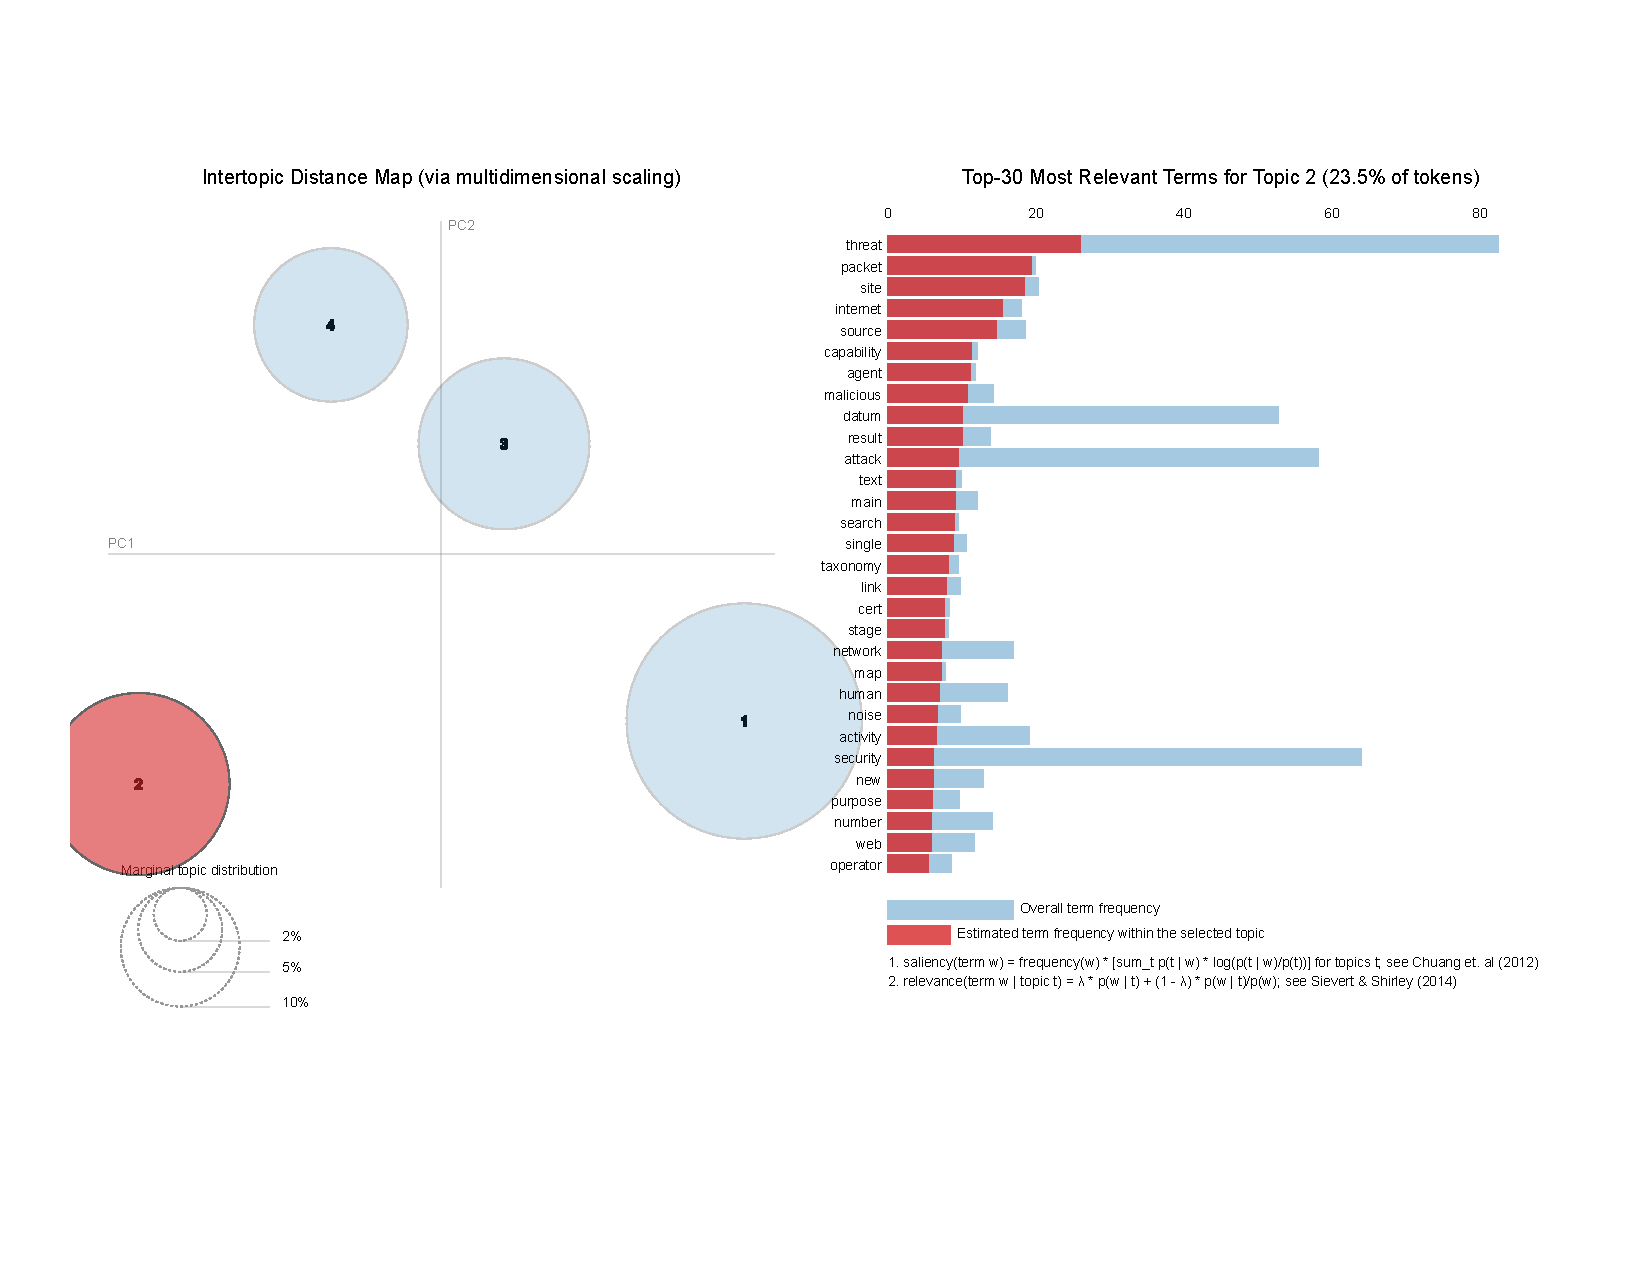
\includegraphics[scale=0.4]{./img/codingALL_topic2.pdf}
\end{center}
\caption{Topic modelling results of the second topic in Surface Web.}
\label{fig:topicmodelling_2}
\end{figure}



%%%%%%%%%%%%%%% %%%%%%%%%%%%%%% 
%%%%%%%%%%%%%%% %%%%%%%%%%%%%%% 
%%%%%%%%%% TABLE topic 3 %%%%%%%%%%%%%%


\begin{table}[h!]
\small
\resizebox{\textwidth}{!}{%
\begin{tabular}{@{}lll@{}}
\toprule
\textbf{Terms} & \textbf{Score} & \textbf{} \\ \midrule 
\rowcolor[HTML]{EFEFEF} 
Process & 7 & \begin{tabular}[c]{@{}l@{}}Processes are all the related activities (parts) inside the system that work together to make it function. \\ A compromised process can lead to a unstable system. In order to compromise a process we have \\ different type of attacks, virus, worm, malware, spyware, trojans. All this attacks have as a target the \\ processes of the system in order to change the main functionalities and make them working for the \\ attacker. In order to avoid this type of attacks is extremely important to have an updated system, a\\ proper antivirus installed and a firewall in order to defend the system environment.\end{tabular} \\
Bitcoin & 4 & \begin{tabular}[c]{@{}l@{}}Bitcoin is either virtual currency or reference to the technology. You can make transactions by check, \\ wiring, or cash. In the last years we witnessed a huge growth of this king of currency and transactions.\\ As a virtual currency, Bitcoins, can also ensure an high level of anonimity and for that reason is widely \\ used for illegal transactions. In the last year we saw bitcoins used for ask ransom after a cyberattack, \\ their extensively use in Dark and Deep web for illegal trafficking and the adoption of this virtual currency\\ in all those activities that need an high level of anonimity.\end{tabular} \\
 &  &  \\
 &  &  \\ \bottomrule
\end{tabular}
}
\caption{Topic analysis results of the third topic for Surface Web.}
\label{tab:topicmodelling_3}
\end{table}


%%%%%%%%%%%%%%% ANALIS TOPIC 3

\begin{figure}
\begin{center}
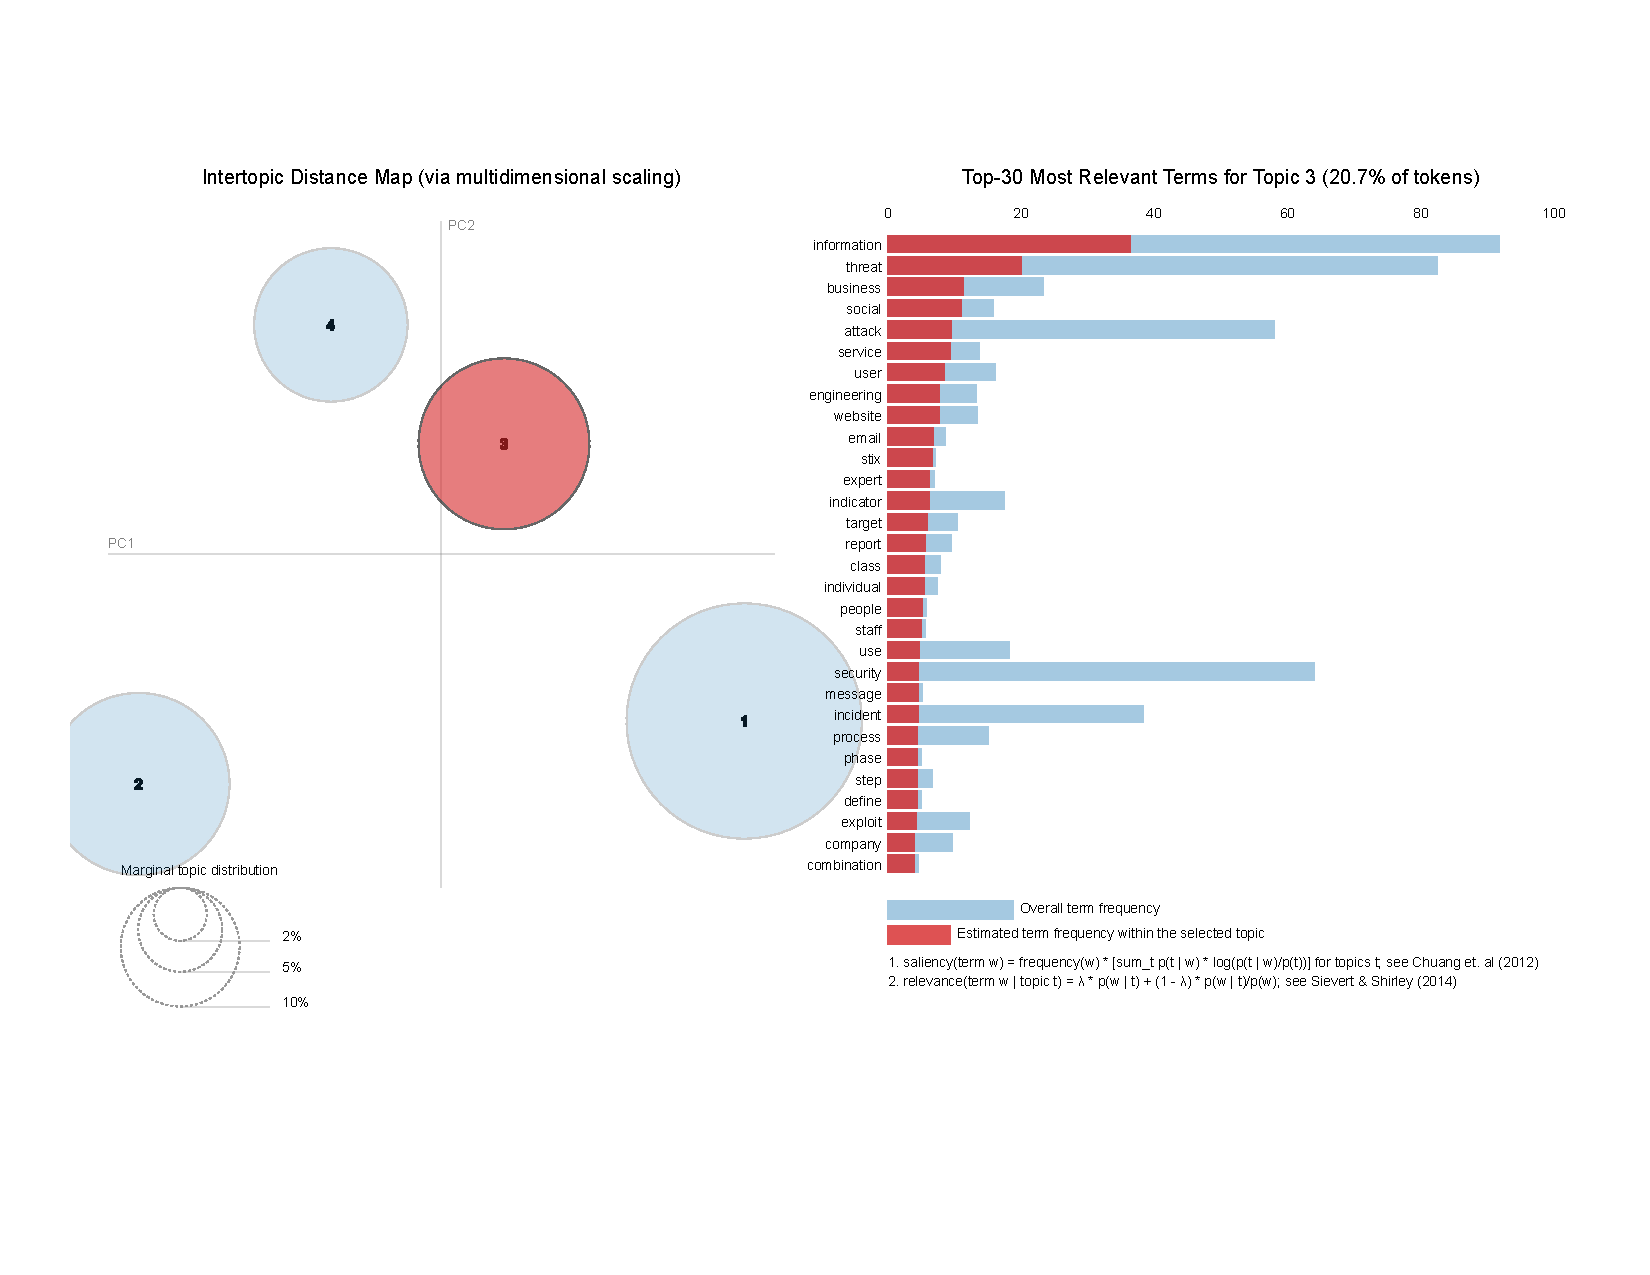
\includegraphics[scale=0.4]{./img/codingALL_topic3.pdf}
\end{center}
\caption{Topic modelling results of the third topic in Surface Web.}
\label{fig:topicmodelling_3}
\end{figure}

%%%%%%%%%%%%%%% %%%%%%%%%%%%%%% 
%%%%%%%%%%%%%%% %%%%%%%%%%%%%%% 
%%%%%%%%%% TABLE topic 4 %%%%%%%%%%%%%%






%%%%%%%%%%%%%%% ANALIS TOPIC 4

\begin{figure}
\begin{center}
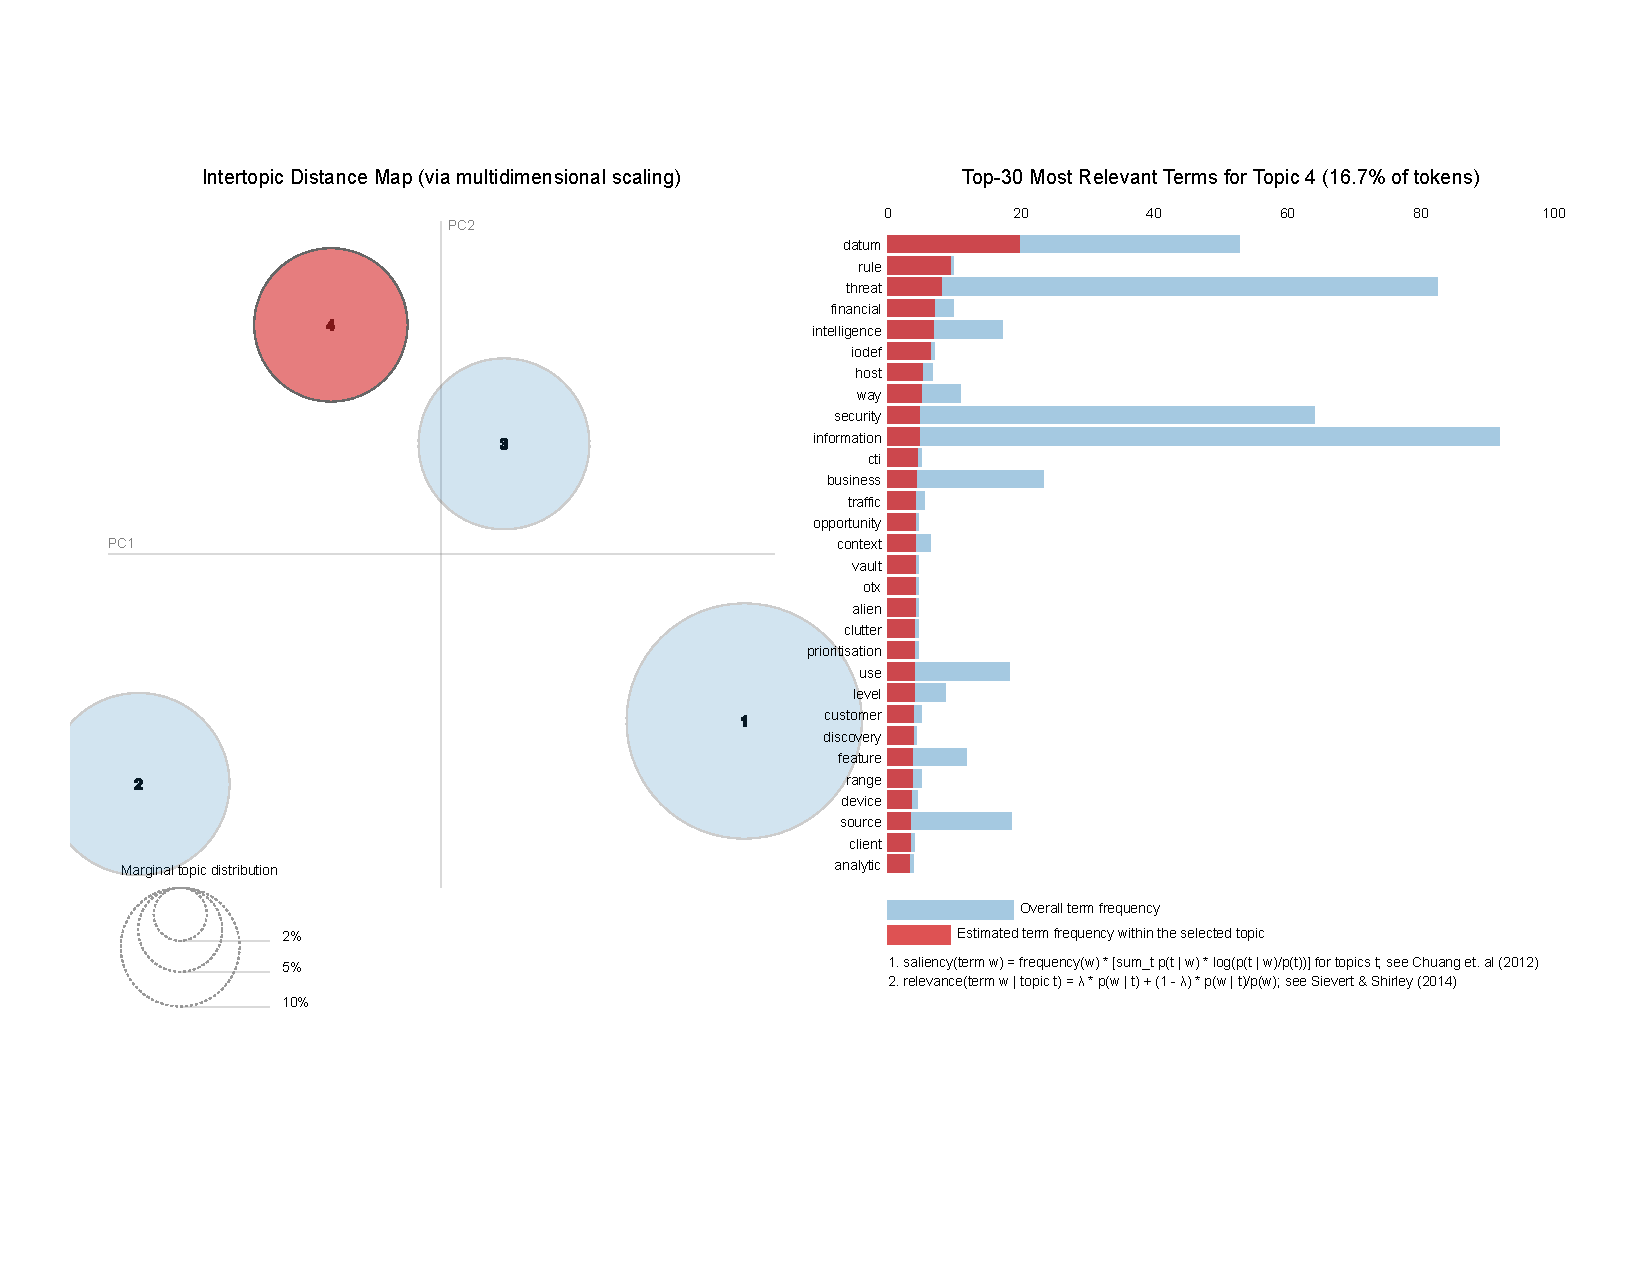
\includegraphics[scale=0.4]{./img/codingALL_topic4.pdf}
\end{center}
\caption{Topic modelling results of the third topic in Surface Web.}
\label{fig:topicmodelling_4}
\end{figure}






\subsubsection{Topic modelling results for Dark and Deep Web}




















\section{Discussion}\label{disc}
\subsection{Answering our Research Questions}

%\begin{itemize}
%\item address each RQ individually (e.g., in a subsubsection?) by stating the RQ and then provide a summary of a response inside a framed box. with a practical impact discussion and target practitioner from academia and elsewhere
%\item offer an example use of the results in the context of each RQ
%\end{itemize}
This section explicitly addresses our research questions. For the sake of space, specifically related research questions (e.g., SRQ1 and SRQ5 as well as SRQ2 and SRQ3) are collapsed into one coherent answer.

\subsubsection{What online depth levels are assessed and to what extent?}

This research question was originally aimed to assess the extent to which the state of the art has targeted exclusively surface, deep, or dark webs respectively and with which technique. Our data indicates a wide array of methods spanning all three levels of depth with sensible overlaps inbetween, e.g., the usage of attack graphs and social-networks analysis of the involved networks. In summary:

\begin{framed}
All depth levels are addressed with a wide range of methods; deep and darkwebs investigation predilects network-based analysis as well as low-level artefact mining (e.g., packet mining, code analysis, etc.).
\end{framed}

\subsubsection{What degrees of anonymity exist for web-crawling?}

This research question was aimed at identify the mechanisms and approaches to ensuring inquirers' anonymity while crawling or analysing the respective network levels shallow, deep, and dark. Our data is rather inconclusive, since many of the approaches (e.g., template avoidance) are only consistent with specific types of investigation. A generalisation of 'degrees' of anonymity is therefore impossible at this stage. In summary:

\begin{framed}
There exists no conclusive crawling/analysis anonymity procedure in the state of the art; this avenue is open for further research opportunity.
\end{framed}

Furthermore, concerning the subsequent research question, namely, ``What policies exist to vary the degrees of anonymity?", there exist relations between the several approaches we did find (e.g., botnets in conjunction with sandboxing as observed in Lauinger et al. \cite{Lauinger2010HoneybotYM}) but there exists no systematic approach to anonymous investigation to date.

\subsubsection{What website features are most indicative of cyberthreats?}

This research question was aimed at identifying the recurrent characteristics and observable features that an online source may be exposing that can be used proactively to identify and profile the criminal activity being perpetrated therein. The data indicates that the indicators are quite varied; on one hand, surface web literature points at using software code features (e.g., responsiveness) as well as their endurance over time (e.g., quality parameters fluctuation). On the other hand, deep and darkweb investigation seems to predilect low-level artefacts e.g., maximum sentence length counts and similar devices. In summary:

\begin{framed}
Surface web analysis literature seems to predilect software code features over appearance metrics for online source risk assessment; conversely, deep and darkweb analysis literature seems to predilect appearance features, e.g., website text content mining.
\end{framed}

%\subsubsection{?}

\subsection{Observations and Lessons Learned}

\begin{itemize}
\item propose a risk-assessment metric?
\item discuss the criminal activity types which were reported in more recent literature?
\item elaborate on crime-specific prediction as well as the emerging criminality types from above?
\item discuss the sparse community working on the topics and the missed convergence between grey and white literature --- offer a descriptive statistic over the community types emerging in the sample and where each result was published to discuss it further.
\end{itemize}

\subsection{Limitations and Threats to Validity}

Based on the taxonomy in \textcolor{red}{\cite{wohlin}, }there are four potential validity threat areas, namely: external, construct, internal, and conclusion validity. 

\emph{ ``External Validity''} concerns the applicability of the results in a more general context. Since our primary studies are obtained from a large extent of disciplines, our results and observations might be only partially applicable to cyber threat intelligence disciplines, this may threaten external validity. To strengthen external-validity, we organized feedback sessions. We analyzed follow-up discussions and used this qualitative data to fine-tune our research methods, and applicability of our results. In addition, we prepared a bundle of all the raw data, all models drawn, all tables, and everything that we used to compose this paper so as to make it available to all who might want to further their understanding on our data (for links see the Appendix). We hope that this can help in making the results and our observations more explicit and applicable in practice.

%Finally,\emph{ ``Instrumental Validity''} concerns the validity of the instruments and methods that were used to conduct the study. Instrumental validity may be threatened since our approach to grounded theory is a hybrid of two methods and might not retain the validity of either. To mitigate these threats we adopted the following counter-measures. To strengthen instrumental-validity, we consulted with grounded theory practitioners and received positive feedback on our method. Also, we consulted additional literature on grounded theory \cite{gtmeth,gtval}. We discovered other hybrids in grounded theory with few claims of invalidation, therefore we assume that our work is as much valid in this sense as others.

\emph{``Construct Validity''} and \emph{``Internal Validity''} concern the generalizability of the constructs under study, as well as the methods used to study and analyze data (e.g. the types of bias involved). To mitigate these threats, we adopted a mixed-methods research approach. On one hand, a formal grounded-theory method was conceived to avoid bias by construction\cite{straussian,gt,gtmeth}. On the other hand, we adopted machine-learning and topic modelling techniques which were appropriately fine-tuned using state of the art approaches to the purpose of elaborating the expected results. As previously explained, to ensure internal and construct validity even further, the initial set of codes for grounded-theory was developed by an external researcher and checked against another external reviewer which is not among the authors and not belonging to the software engineering field. In addition we applied grounded-theory in two rounds: (a) first the primary studies were split across a group of students, to apply grounded theory; (b) in the second round one of the authors re-executed a blind grounded-theory on the full primary studies set. When both rounds were finished, both grounded-theories were analyzed evenly to construct a unique theory. When disagreement between the two samples was found, a session was organized with students researchers and supervisors to examine the samples and check them against literature.

%from which were designed to reduce author bias to a minimum. Moreover, the coding and initial theory generation were carried out twice: first by a group of Masters' Students and then by one of the authors from scratch. Both samples were used evenly to generate a theory. Finally the theory was checked by two supervising researchers.

\emph{``Conclusion Validity''} concerns the degree to which our conclusions are reasonable based on our data. The logical reasoning behind our conclusions are dictated by sound analysis of the data through grounded theory and other analysis methods which try and construct theory from data rather than confirming initial hypotheses, as explained in \cite{gtmeth,gtval}. Moreover, all the conclusions in this paper were drawn by three researchers and double-checked against data, primary papers or related studies. 

\section{Conclusions}\label{conc}
%\begin{enumerate}
%\item recap of what we did, tailor and modify from the intro
%\item address each research question with each of the results and pointers to the relative sections; discuss here the impact and practical uses
%\item elaborate on practical impact, final considerations (what's missing) 
%\item future work?
%\end{enumerate}

This paper provides a Systematic Multi-Vocal Literature Review on the methods, indicators, approaches and techniques previously explored for the purpose of cybercrime threat intelligence, namely, the act of gathering information over, predicting, avoiding, or prosecuting cyber-criminal activities in the surface-, deep-, and dark-webs. More specifically, the attained results provide an overview of the state of the art over (a) what online depth levels are assessed and to what extent; (b) what degrees of anonymity exist for web-crawling; (c) what policies exist to vary the degrees of anonymity; (d) what website features are most indicative of cyberthreats; (e) what risk assessment techniques exist.

Overall, our data, results, and discussions support three conclusions.

First, there is a distinct gap between the grey literature --- which mainly discusses reported vulnerabilities as well as organisational/economical/financial consequences of being targeted by cybercriminal activity --- and the white research literature --- which mainly focuses on offering scattered non-definitive attempts at predicting, avoiding, or protecting against specific criminal-activity types. To address this gap, we discussed our results and the limitations therein, also offering a preliminary formulation of a holistic metric to assess the risk-level that any given online source may be theatre to online criminal activity.

Second, no single community encapsulates cybercrime-fighting software, tools, approaches and techniques, rather, these techniques or their relevant related work is scattered across as many as 30+ domain-specific communities (e.g., software security, data privacy, software engineering, distributed computing, artificial intelligence, and more). In discussing this observation we offered descriptive statistics over our sample in the hope of pointing community leaders in the right direction while fostering cross-fertilisation or community-building.

Third, finally, there is no one definitive solution towards assisting law-enforcement agencies in their cybercrime-fighting activity. A holistic integration effort is advised.



In the future we plan to address the above shortcomings even further, to the extent that, (1) we aim at providing a holistic tool to aid law-enforcers in combatting and prosecuting online criminal activity, (2) we aim at fostering a data-driven, cybercrime-fighting practitioners community and (3) most immediately, we aim at building a tool for large-scale online datasource risk-assessment of criminal activity. We plan to conduct and refine the above activities in the scope of the EU ANITA H2020 project in direct synergy with the law-enforcement practitioners within the ANITA consortium.

\begin{acks}
The work is supported by the EU H2020  framework programme, grant ``ANITA" under Grant No.: 787061 and grant ``PRoTECT" under Grant No.: 815356.
\end{acks}

% Bibliography
\bibliographystyle{ACM-Reference-Format}
\bibliography{newbib}



\end{document}
